% !TEX program = pdflatex
\documentclass[a4paper,14pt]{extarticle}

% ===== Язык и кодировка =====
\usepackage[T2A]{fontenc}
\usepackage[utf8]{inputenc}
\usepackage[russian,english]{babel}

% ===== Поля =====
\usepackage[left=30mm, right=15mm, top=20mm, bottom=20mm]{geometry}

% ===== Графика и таблицы =====
\usepackage{graphicx}
\usepackage{longtable}
\usepackage{array}
\usepackage{booktabs}
\usepackage{tabularx}
\usepackage{float}
\usepackage{pdflscape}

% ===== Листинги кода =====
\usepackage{listings}
\usepackage{etoolbox}

\lstset{
  inputencoding=utf8,
  extendedchars=true,
  keepspaces=true,
  literate=
   {а}{{\selectfont\char224}}1 {б}{{\selectfont\char225}}1
   {в}{{\selectfont\char226}}1 {г}{{\selectfont\char227}}1
   {д}{{\selectfont\char228}}1 {е}{{\selectfont\char229}}1
   {ё}{{\"e}}1
   {ж}{{\selectfont\char230}}1 {з}{{\selectfont\char231}}1
   {и}{{\selectfont\char232}}1 {й}{{\selectfont\char233}}1
   {к}{{\selectfont\char234}}1 {л}{{\selectfont\char235}}1
   {м}{{\selectfont\char236}}1 {н}{{\selectfont\char237}}1
   {о}{{\selectfont\char238}}1 {п}{{\selectfont\char239}}1
   {р}{{\selectfont\char240}}1 {с}{{\selectfont\char241}}1
   {т}{{\selectfont\char242}}1 {у}{{\selectfont\char243}}1
   {ф}{{\selectfont\char244}}1 {х}{{\selectfont\char245}}1
   {ц}{{\selectfont\char246}}1 {ч}{{\selectfont\char247}}1
   {ш}{{\selectfont\char248}}1 {щ}{{\selectfont\char249}}1
   {ъ}{{\selectfont\char250}}1 {ы}{{\selectfont\char251}}1
   {ь}{{\selectfont\char252}}1 {э}{{\selectfont\char253}}1
   {ю}{{\selectfont\char254}}1 {я}{{\selectfont\char255}}1
   {А}{{\selectfont\char192}}1 {Б}{{\selectfont\char193}}1
   {В}{{\selectfont\char194}}1 {Г}{{\selectfont\char195}}1
   {Д}{{\selectfont\char196}}1 {Е}{{\selectfont\char197}}1
   {Ё}{{\"E}}1
   {Ж}{{\selectfont\char198}}1 {З}{{\selectfont\char199}}1
   {И}{{\selectfont\char200}}1 {Й}{{\selectfont\char201}}1
   {К}{{\selectfont\char202}}1 {Л}{{\selectfont\char203}}1
   {М}{{\selectfont\char204}}1 {Н}{{\selectfont\char205}}1
   {О}{{\selectfont\char206}}1 {П}{{\selectfont\char207}}1
   {Р}{{\selectfont\char208}}1 {С}{{\selectfont\char209}}1
   {Т}{{\selectfont\char210}}1 {У}{{\selectfont\char211}}1
   {Ф}{{\selectfont\char212}}1 {Х}{{\selectfont\char213}}1
   {Ц}{{\selectfont\char214}}1 {Ч}{{\selectfont\char215}}1
   {Ш}{{\selectfont\char216}}1 {Щ}{{\selectfont\char217}}1
   {Ъ}{{\selectfont\char218}}1 {Ы}{{\selectfont\char219}}1
   {Ь}{{\selectfont\char220}}1 {Э}{{\selectfont\char221}}1
   {Ю}{{\selectfont\char222}}1 {Я}{{\selectfont\char223}}1
}

\usepackage{xcolor}
\usepackage{fancyvrb}

\colorlet{lststringcolor}{red!70!black}

\lstset{
  language=C,
  basicstyle=\footnotesize\ttfamily,
  keywordstyle=\color{blue}\bfseries,
  commentstyle=\color{gray}\itshape,
  stringstyle=\color{lststringcolor},
  numbers=left,
  numberstyle=\tiny\color{gray},
  numbersep=8pt,
  frame=single,
  breaklines=true,
  breakatwhitespace=false,
  columns=fullflexible,
  tabsize=4,
  showstringspaces=false,
  captionpos=b,
  postbreak=\mbox{$\hookrightarrow$\space},
}

% ===== Блок сложности =====
\newcommand{\opcount}[2]{%
  \par\vspace{2pt}%
  \noindent
  \colorbox{gray!15}{%
    \parbox{\dimexpr\linewidth-2\fboxsep\relax}{%
      \small\bfseries\ttfamily\raggedright #1:\enskip #2%
    }%
  }%
  \par\vspace{6pt}%
}

% ===== Гиперссылки =====
\PassOptionsToPackage{hyphens}{url}
\usepackage{amsmath}
\usepackage{hyperref}
\hypersetup{
  colorlinks=true,
  linkcolor=black,
  urlcolor=blue,
  citecolor=black,
}

% ===== Отступ первого абзаца =====
\usepackage{indentfirst}
\setlength{\parindent}{1.25cm}

% ===== Межстрочный интервал =====
\usepackage{setspace}
\onehalfspacing

% ===== Заголовки разделов =====
\usepackage{titlesec}
\titleformat{\section}{\normalfont\large\bfseries\centering}{\thesection.}{0.5em}{}
\titleformat{\subsection}{\normalfont\normalsize\bfseries}{\thesubsection.}{0.5em}{}

% ===== Перенос слов =====
\usepackage{ragged2e}
\emergencystretch=6em
\tolerance=9999
\hbadness=10001

\DeclareUrlCommand\code{\urlstyle{tt}}
\newcommand{\tcode}[1]{\code{#1}}

% ===== Подписи рисунков =====
\usepackage{caption}
\captionsetup{justification=centering, labelsep=endash}

\begin{document}

% ===================== ТИТУЛЬНЫЙ ЛИСТ =====================
\begin{titlepage}
\begin{center}

\textbf{Национальный исследовательский университет ИТМО}\\[0.5cm]
\textbf{Факультет безопасности информационных технологий}\\[2cm]

{\Large\textbf{Алгоритмы и структуры данных}}\\[1cm]
{\large Лабораторная работа №3}\\[0.5cm]
{\large\textbf{<<Цифровая сортировка дека с поиском методом Райта>>}}\\[3cm]

\begin{flushright}
\begin{minipage}{0.45\textwidth}
\textbf{Выполнил:}\\
Студент группы N3247\\
Сивоконь А.А.\\[1cm]

\noindent\rule{6cm}{0.4pt}\\
\centerline{(подпись)}

\vspace{0.5cm}

\textbf{Преподаватель:}\\
Ерофеев С.А.\\[1cm]
\noindent\rule{6cm}{0.4pt}\\
\centerline{(отметка о выполнении)}

\vspace{1.5cm}

\noindent\rule{6cm}{0.4pt}\\
\centerline{(подпись)}
\end{minipage}
\end{flushright}

\vfill

Санкт-Петербург\\
2026

\end{center}
\end{titlepage}

% ===================== СОДЕРЖАНИЕ =====================
\newpage
\renewcommand{\contentsname}{Содержание}
\tableofcontents

% ===================== 1. ПОСТАНОВКА ЗАДАЧИ =====================
\newpage
\section{Постановка задачи}

\textbf{Цель работы:} разработать программу цифровой сортировки (Radix Sort LSD) для последовательности целых чисел (включая отрицательные), считываемых из файла, используя в качестве основной и вспомогательной структуры данных \textbf{дек на основе двусвязного списка}; реализовать \textbf{поиск методом Райта} в отсортированном деке; определить сложность программы.

\vspace{0.5cm}
\textbf{Для достижения поставленной цели необходимо решить следующие задачи:}
\begin{enumerate}
  \item Реализовать дек на двусвязном списке с операциями \texttt{push\_front}, \texttt{push\_back}, \texttt{pop\_front}, \texttt{pop\_back}, \texttt{deque\_is\_empty}, \texttt{deque\_free};
  \item Реализовать чтение последовательности целых чисел из файла непосредственно в дек;
  \item Реализовать алгоритм цифровой сортировки LSD через 10 деков-корзин;
  \item Корректно обработать отрицательные числа: разделить дек на два вспомогательных, отсортировать каждый независимо, объединить результат;
  \item Реализовать поиск методом Райта в отсортированном деке;
  \item Оценить теоретическую сложность алгоритмов;
  \item Провести тестирование программы на различных наборах данных;
  \item Составить блок-схемы алгоритма и оформить отчёт.
\end{enumerate}

% ===================== 2. ОПИСАНИЕ СТРУКТУР И АЛГОРИТМОВ =====================
\newpage
\section{Описание структур данных и алгоритмов}

\subsection{Дек на двусвязном списке}

Основной структурой данных является дек (двусторонняя очередь) на основе динамически выделяемых узлов двусвязного списка:

\begin{itemize}
  \item Узел \texttt{DNode} содержит значение \texttt{value} и два указателя: \texttt{prev} (на предыдущий узел) и \texttt{next} (на следующий).
  \item Дек \texttt{Deque} хранит указатели \texttt{front} (голова) и \texttt{back} (хвост), а также счётчик \texttt{size}. Двусвязность обеспечивает $O(1)$ для вставки и удаления \textit{с обоих концов}, что необходимо как для сортировки, так и для поиска методом Райта.
  \item При добавлении первого элемента он становится одновременно головой и хвостом: оба указателя \texttt{front} и \texttt{back} ссылаются на него.
\end{itemize}

\textbf{Операции дека:}

\begin{center}
\begin{tabular}{|l|l|}
\hline
\textbf{Функция} & \textbf{Описание} \\
\hline
\texttt{deque\_init}      & обнулить поля \texttt{front}, \texttt{back}, \texttt{size} \\
\hline
\texttt{deque\_is\_empty} & вернуть \texttt{size==0}                                   \\
\hline
\texttt{push\_front}      & добавить элемент в голову                                  \\
\hline
\texttt{push\_back}       & добавить элемент в хвост                                   \\
\hline
\texttt{pop\_front}       & извлечь элемент из головы                                  \\
\hline
\texttt{pop\_back}        & извлечь элемент из хвоста                                  \\
\hline
\texttt{deque\_free}      & освободить все узлы                                        \\
\hline
\end{tabular}
\end{center}

\subsection{Алгоритм цифровой сортировки LSD}

Цифровая сортировка~--- нерекурсивный алгоритм, обрабатывающий числа поразрядно от \textit{младшего} разряда к \textit{старшему} (LSD~--- Least Significant Digit).

\textbf{Пошаговый алгоритм функции \tcode{counting_sort_by_deque}:}

\begin{enumerate}
  \item \textbf{Шаг 1.} Инициализировать 10 деков-корзин \texttt{buckets[0..9]}.
  \item \textbf{Шаг 2.} Пока исходный дек не пуст: извлечь элемент через \texttt{pop\_front}, вычислить цифру текущего разряда \texttt{(v\,/\,exp)\,\%\,10}, добавить элемент в \texttt{buckets[digit]} через \texttt{push\_back}.
  \item \textbf{Шаг 3.} Обходя корзины \texttt{buckets[0..9]} по порядку: пока корзина не пуста, извлекать элементы через \texttt{pop\_front} и добавлять обратно в исходный дек через \texttt{push\_back}. Порядок FIFO (добавление в хвост, извлечение из головы) гарантирует устойчивость сортировки.
\end{enumerate}

\textbf{Поддержка отрицательных чисел.} Функция \texttt{radix\_sort} разделяет исходный дек на два вспомогательных: \texttt{neg}~--- модули отрицательных чисел, \texttt{pos}~--- неотрицательные числа. Каждый дек сортируется независимо через \texttt{radix\_sort\_nonneg}. При сборе результата из \texttt{neg} элементы извлекаются с~\textit{хвоста} (\texttt{pop\_back})~--- потому что наибольший модуль соответствует наименьшему отрицательному числу,~--- и добавляются со знаком минус. Затем добавляются элементы из \texttt{pos} с~головы (\texttt{pop\_front}).

\subsection{Поиск методом Райта}

Поиск методом Райта предназначен для работы с \textit{упорядоченным} двусвязным списком и позволяет в среднем вдвое сократить число сравнений по сравнению с линейным поиском от головы.

\textbf{Алгоритм функции \texttt{wright\_search}:}

\begin{enumerate}
  \item \textbf{Шаг 1. Выход на середину.} От головы дека выполнить $\lfloor n/2 \rfloor$ шагов по указателю \texttt{next}~--- получить указатель на средний элемент. На этом шаге сравнения с ключом не производятся.
  \item \textbf{Шаг 2. Сравнение с серединой.} Если \texttt{key == cur->value}~--- элемент найден.
  \item \textbf{Шаг 3. Направленное движение.} Если $\texttt{key} < \texttt{cur->value}$~--- двигаться по \texttt{prev} влево, пока \texttt{cur->value > key}. Иначе~--- двигаться по \texttt{next} вправо, пока \texttt{cur->value < key}. Условие раннего выхода следует из упорядоченности: ключ заведомо отсутствует в оставшейся части.
  \item \textbf{Шаг 4. Проверка точки остановки.} Если остановились на узле с \texttt{cur->value == key}~--- найден; иначе~--- отсутствует.
\end{enumerate}

\textbf{Почему необходим двусвязный список.} Шаг~3 требует движения от середины как влево (по \texttt{prev}), так и вправо (по \texttt{next}). Односвязный список не позволяет двигаться назад, поэтому метод Райта применим только к двусвязной структуре.

\subsection{Маршрут программы}

\begin{enumerate}
  \item \textbf{Чтение входного файла} (\texttt{read\_file}): однопроходное считывание чисел из файла непосредственно в дек через \texttt{push\_back}.
  \item \textbf{Вывод исходного дека} (\texttt{deque\_print}).
  \item \textbf{Выполнение Radix Sort} (\texttt{radix\_sort}): разделение на отрицательные/неотрицательные, сортировка, объединение.
  \item \textbf{Вывод отсортированного дека} (\texttt{deque\_print}).
  \item \textbf{Поиск методом Райта} (\texttt{wright\_search}): ключи задаются аргументами командной строки или вводятся с клавиатуры.
  \item \textbf{Освобождение памяти}: \texttt{deque\_free}.
\end{enumerate}

% ===================== 3. ОПИСАНИЕ ПЕРЕМЕННЫХ =====================
\newpage
\section{Описание используемых переменных}

В таблице~\ref{tab:vars} приведено описание переменных программы.

\captionsetup[longtable]{name={Таблица}}
\newcolumntype{L}[1]{>{\RaggedRight\arraybackslash}p{#1}}

\begin{longtable}{|L{3.4cm}|L{3.0cm}|L{3.6cm}|L{4.5cm}|}
\caption{Описание переменных программы}\label{tab:vars}\\
\hline
\textbf{Переменная} & \textbf{Тип} & \textbf{Границы} & \textbf{Назначение} \\
\hline
\endfirsthead
\hline
\textbf{Переменная} & \textbf{Тип} & \textbf{Границы} & \textbf{Назначение} \\
\hline
\endhead
\hline
\endfoot

\multicolumn{4}{|c|}{\textbf{Главная программа (main.c)}} \\
\hline
filename   & \texttt{const char*}  & строка               & Имя входного файла \\
\hline
d          & \texttt{Deque}        & структура            & Основной дек программы \\
\hline
n          & \texttt{int}          & $[1;\;2^{31}-1]$     & Количество прочитанных чисел \\
\hline
key        & \texttt{int}          & любое целое          & Ключ поиска \\
\hline
pos        & \texttt{int}          & $[-1;\;n-1]$         & Позиция найденного элемента \\
\hline
views      & \texttt{int}          & $[0;\;n]$            & Число просмотров при поиске \\
\hline
node       & \texttt{const DNode*} & адрес / NULL         & Результат поиска Райта \\
\hline

\multicolumn{4}{|c|}{\textbf{Узел и дек (deque.c)}} \\
\hline
DNode.value & \texttt{int}         & любое целое          & Хранимое значение \\
\hline
DNode.prev  & \texttt{DNode*}      & адрес / NULL         & Указатель на предыдущий узел \\
\hline
DNode.next  & \texttt{DNode*}      & адрес / NULL         & Указатель на следующий узел \\
\hline
Deque.front & \texttt{DNode*}      & адрес / NULL         & Голова дека \\
\hline
Deque.back  & \texttt{DNode*}      & адрес / NULL         & Хвост дека \\
\hline
Deque.size  & \texttt{int}         & $[0;\;n]$            & Текущий размер дека \\
\hline
cur         & \texttt{DNode*}      & адрес / NULL         & Текущий узел при обходе \\
\hline

\multicolumn{4}{|c|}{\textbf{Ввод из файла (deque.c)}} \\
\hline
fp          & \texttt{FILE*}       & адрес                & Указатель на открытый файл \\
\hline
tmp         & \texttt{int}         & любое целое          & Очередное считанное число \\
\hline

\multicolumn{4}{|c|}{\textbf{Цифровая сортировка (deque.c)}} \\
\hline
exp         & \texttt{int}         & $\{1,\,10,\,\ldots,\,10^{d-1}\}$ & Текущий разряд \\
\hline
buckets[10] & \texttt{Deque[10]}   & ---                  & Десять деков-корзин \\
\hline
digit       & \texttt{int}         & $[0;\;9]$            & Цифра текущего разряда \\
\hline
max\_val    & \texttt{int}         & $[0;\;2^{31}-1]$     & Максимум для определения $d$ \\
\hline
neg         & \texttt{Deque}       & структура            & Дек модулей отрицательных чисел \\
\hline
pos         & \texttt{Deque}       & структура            & Дек неотрицательных чисел \\
\hline
value       & \texttt{int}         & любое целое          & Временная при pop/push \\
\hline

\multicolumn{4}{|c|}{\textbf{Поиск методом Райта (deque.c)}} \\
\hline
mid         & \texttt{int}         & $[0;\;n/2]$          & Индекс среднего элемента \\
\hline
idx         & \texttt{int}         & $[0;\;n-1]$          & Текущая позиция при обходе \\
\hline
cur         & \texttt{const DNode*}& адрес / NULL         & Текущий узел при поиске \\
\hline

\end{longtable}

% ===================== 4. ТЕСТИРОВАНИЕ =====================
\newpage
\section{Тестирование программы}

\subsection{Тест 1: стандартная сортировка и поиск}

Файл \texttt{input.txt}: \texttt{170 45 75 90 802 24 2 66 -73 -4}

\begin{Verbatim}[frame=single,fontsize=\footnotesize]
$ ./sort input.txt 75 2 802

Чтение файла 'input.txt'...
Прочитано 10 чисел.

Исходный дек:
170 45 75 90 802 24 2 66 -73 -4

Выполняем цифровую сортировку дека...
Отсортированный дек:
-73 -4 2 24 45 66 75 90 170 802

── Поиск методом Райта ──────────────────────────
Ключ 75: НАЙДЕН на позиции 6 (просмотров: 2)
Ключ 2: НАЙДЕН на позиции 2 (просмотров: 4)
Ключ 802: НАЙДЕН на позиции 9 (просмотров: 5)
─────────────────────────────────────────────────
\end{Verbatim}

Дек успешно отсортирован. Все три ключа найдены. Для ключа~75 (позиция~6): средний элемент на позиции~5 равен~66~$<$~75, поэтому поиск сдвигается вправо~--- найдено за 2~просмотра.

\subsection{Тест 2: дек с отрицательными числами}

Входной файл \texttt{neg.txt}: \texttt{-15 3 -7 42 -2 18}

\begin{Verbatim}[frame=single,fontsize=\footnotesize]
$ ./sort neg.txt -15 5

Чтение файла 'neg.txt'...
Прочитано 6 чисел.

Исходный дек:
-15 3 -7 42 -2 18

Выполняем цифровую сортировку дека...
Отсортированный дек:
-15 -7 -2 3 18 42

── Поиск методом Райта ──────────────────────────
Ключ -15: НАЙДЕН на позиции 0 (просмотров: 4)
Ключ 5: не найден (просмотров: 2)
─────────────────────────────────────────────────
\end{Verbatim}

Программа корректно разделила дек на \texttt{neg}~$=\{15, 7, 2\}$ (по модулю) и \texttt{pos}~$=\{3, 42, 18\}$, отсортировала каждый и собрала результат: сначала отрицательные в порядке возрастания $(-15, -7, -2)$, затем положительные $(3, 18, 42)$.

\subsection{Тест 3: дек из одного элемента}

\begin{Verbatim}[frame=single,fontsize=\footnotesize]
$ ./sort one.txt 5 9

Чтение файла 'one.txt'...
Прочитано 1 число.

Исходный дек:
5

Выполняем цифровую сортировку дека...
Отсортированный дек:
5

── Поиск методом Райта ──────────────────────────
Ключ 5: НАЙДЕН на позиции 0 (просмотров: 1)
Ключ 9: не найден (просмотров: 1)
─────────────────────────────────────────────────
\end{Verbatim}

Граничный случай: сортировка возвращает управление сразу (менее двух элементов). Поиск обоих ключей завершается за 1~просмотр (середина~--- единственный элемент).

\subsection{Тест 4: несуществующий файл}

\begin{Verbatim}[frame=single,fontsize=\footnotesize]
$ ./sort missing.txt
Чтение файла 'missing.txt'...
Ошибка: не удалось открыть файл 'missing.txt'
\end{Verbatim}

Программа корректно обрабатывает ошибку открытия файла и завершает работу с кодом \texttt{EXIT\_FAILURE}.

\subsection{Тест 5: пустой файл}

\begin{Verbatim}[frame=single,fontsize=\footnotesize]
$ ./sort empty.txt
Чтение файла 'empty.txt'...
Ошибка: файл 'empty.txt' пуст или не содержит чисел
\end{Verbatim}

Программа корректно обнаруживает пустой файл и завершает работу с кодом \texttt{EXIT\_FAILURE}.

% ===================== 5. БЛОК-СХЕМЫ =====================
\newpage
\section{Блок-схемы алгоритма}

Блок-схемы всех подпрограмм приведены в Приложении~А (стр.~\pageref{sec:appendix}).

Перечень блок-схем:
\begin{enumerate}
  \item Главная программа (\texttt{main})
  \item Чтение из файла (\texttt{read\_file})
  \item Цифровая сортировка (\texttt{radix\_sort})
  \item Сортировка по разряду через деки (\tcode{counting_sort_by_deque})
  \item Добавление в голову дека (\texttt{push\_front})
  \item Добавление в хвост дека (\texttt{push\_back})
  \item Извлечение из головы дека (\texttt{pop\_front})
  \item Извлечение из хвоста дека (\texttt{pop\_back})
  \item Поиск методом Райта (\texttt{wright\_search})
\end{enumerate}

% ===================== 6. ИСХОДНЫЙ КОД =====================
\newpage
\section{Исходный код программы}

Программа состоит из трёх файлов: \texttt{deque.h}~--- объявления структур и всех функций; \texttt{deque.c}~--- реализация дека, алгоритма сортировки и поиска методом Райта; \texttt{main.c}~--- точка входа, ввод/вывод.

\subsection{Файл deque.h}

\lstinputlisting[language=C]{deque.h}

\subsection{Файл deque.c}

\subsubsection*{Операции дека}

\lstinputlisting[language=C, firstline=1, lastline=132]{deque.c}

\subsubsection*{Цифровая сортировка}

\lstinputlisting[language=C, firstline=134, lastline=228]{deque.c}

\subsubsection*{Поиск методом Райта}

\lstinputlisting[language=C, firstline=230, lastline=290]{deque.c}

\subsection{Файл main.c}

\lstinputlisting[language=C]{main.c}

% ===================== ЗАКЛЮЧЕНИЕ =====================
\newpage
\section*{Заключение}
\addcontentsline{toc}{section}{Заключение}

В ходе выполнения лабораторной работы была разработана программа на языке~C, реализующая цифровую сортировку LSD целых чисел (включая отрицательные), считываемых из файла, с использованием \textbf{дека на основе двусвязного списка} в качестве основной и вспомогательной структуры данных, а также \textbf{поиск методом Райта} в отсортированном деке.

Программа организована в три файла: \texttt{deque.h} объявляет структуры и интерфейс; \texttt{deque.c} реализует дек, сортировку и поиск; \texttt{main.c} содержит точку входа и ввод/вывод.

Поддержка отрицательных чисел реализована через разделение дека на два вспомогательных (модули отрицательных и положительные), их независимую сортировку и сборку результата: из \texttt{neg} элементы извлекаются с хвоста (чтобы сохранить порядок), из \texttt{pos}~--- с головы.

Поиск методом Райта использует двусвязность списка: стартует со среднего элемента и движется по \texttt{prev} или \texttt{next} в зависимости от соотношения ключа со средним значением.

Результаты тестирования подтверждают корректность сортировки для всех рассмотренных случаев~--- стандартного, с отрицательными числами, с одним элементом~--- а также правильную обработку ошибочных ситуаций.

% ===================== ПРИЛОЖЕНИЕ А =====================
\clearpage
\phantomsection
\label{sec:appendix}
\section*{Приложение А. Блок-схемы алгоритма}
\addcontentsline{toc}{section}{Приложение А. Блок-схемы алгоритма}

\renewcommand{\figurename}{Рис.}

\begin{landscape}

\begin{figure}[H]
\centering
\makebox[\linewidth][c]{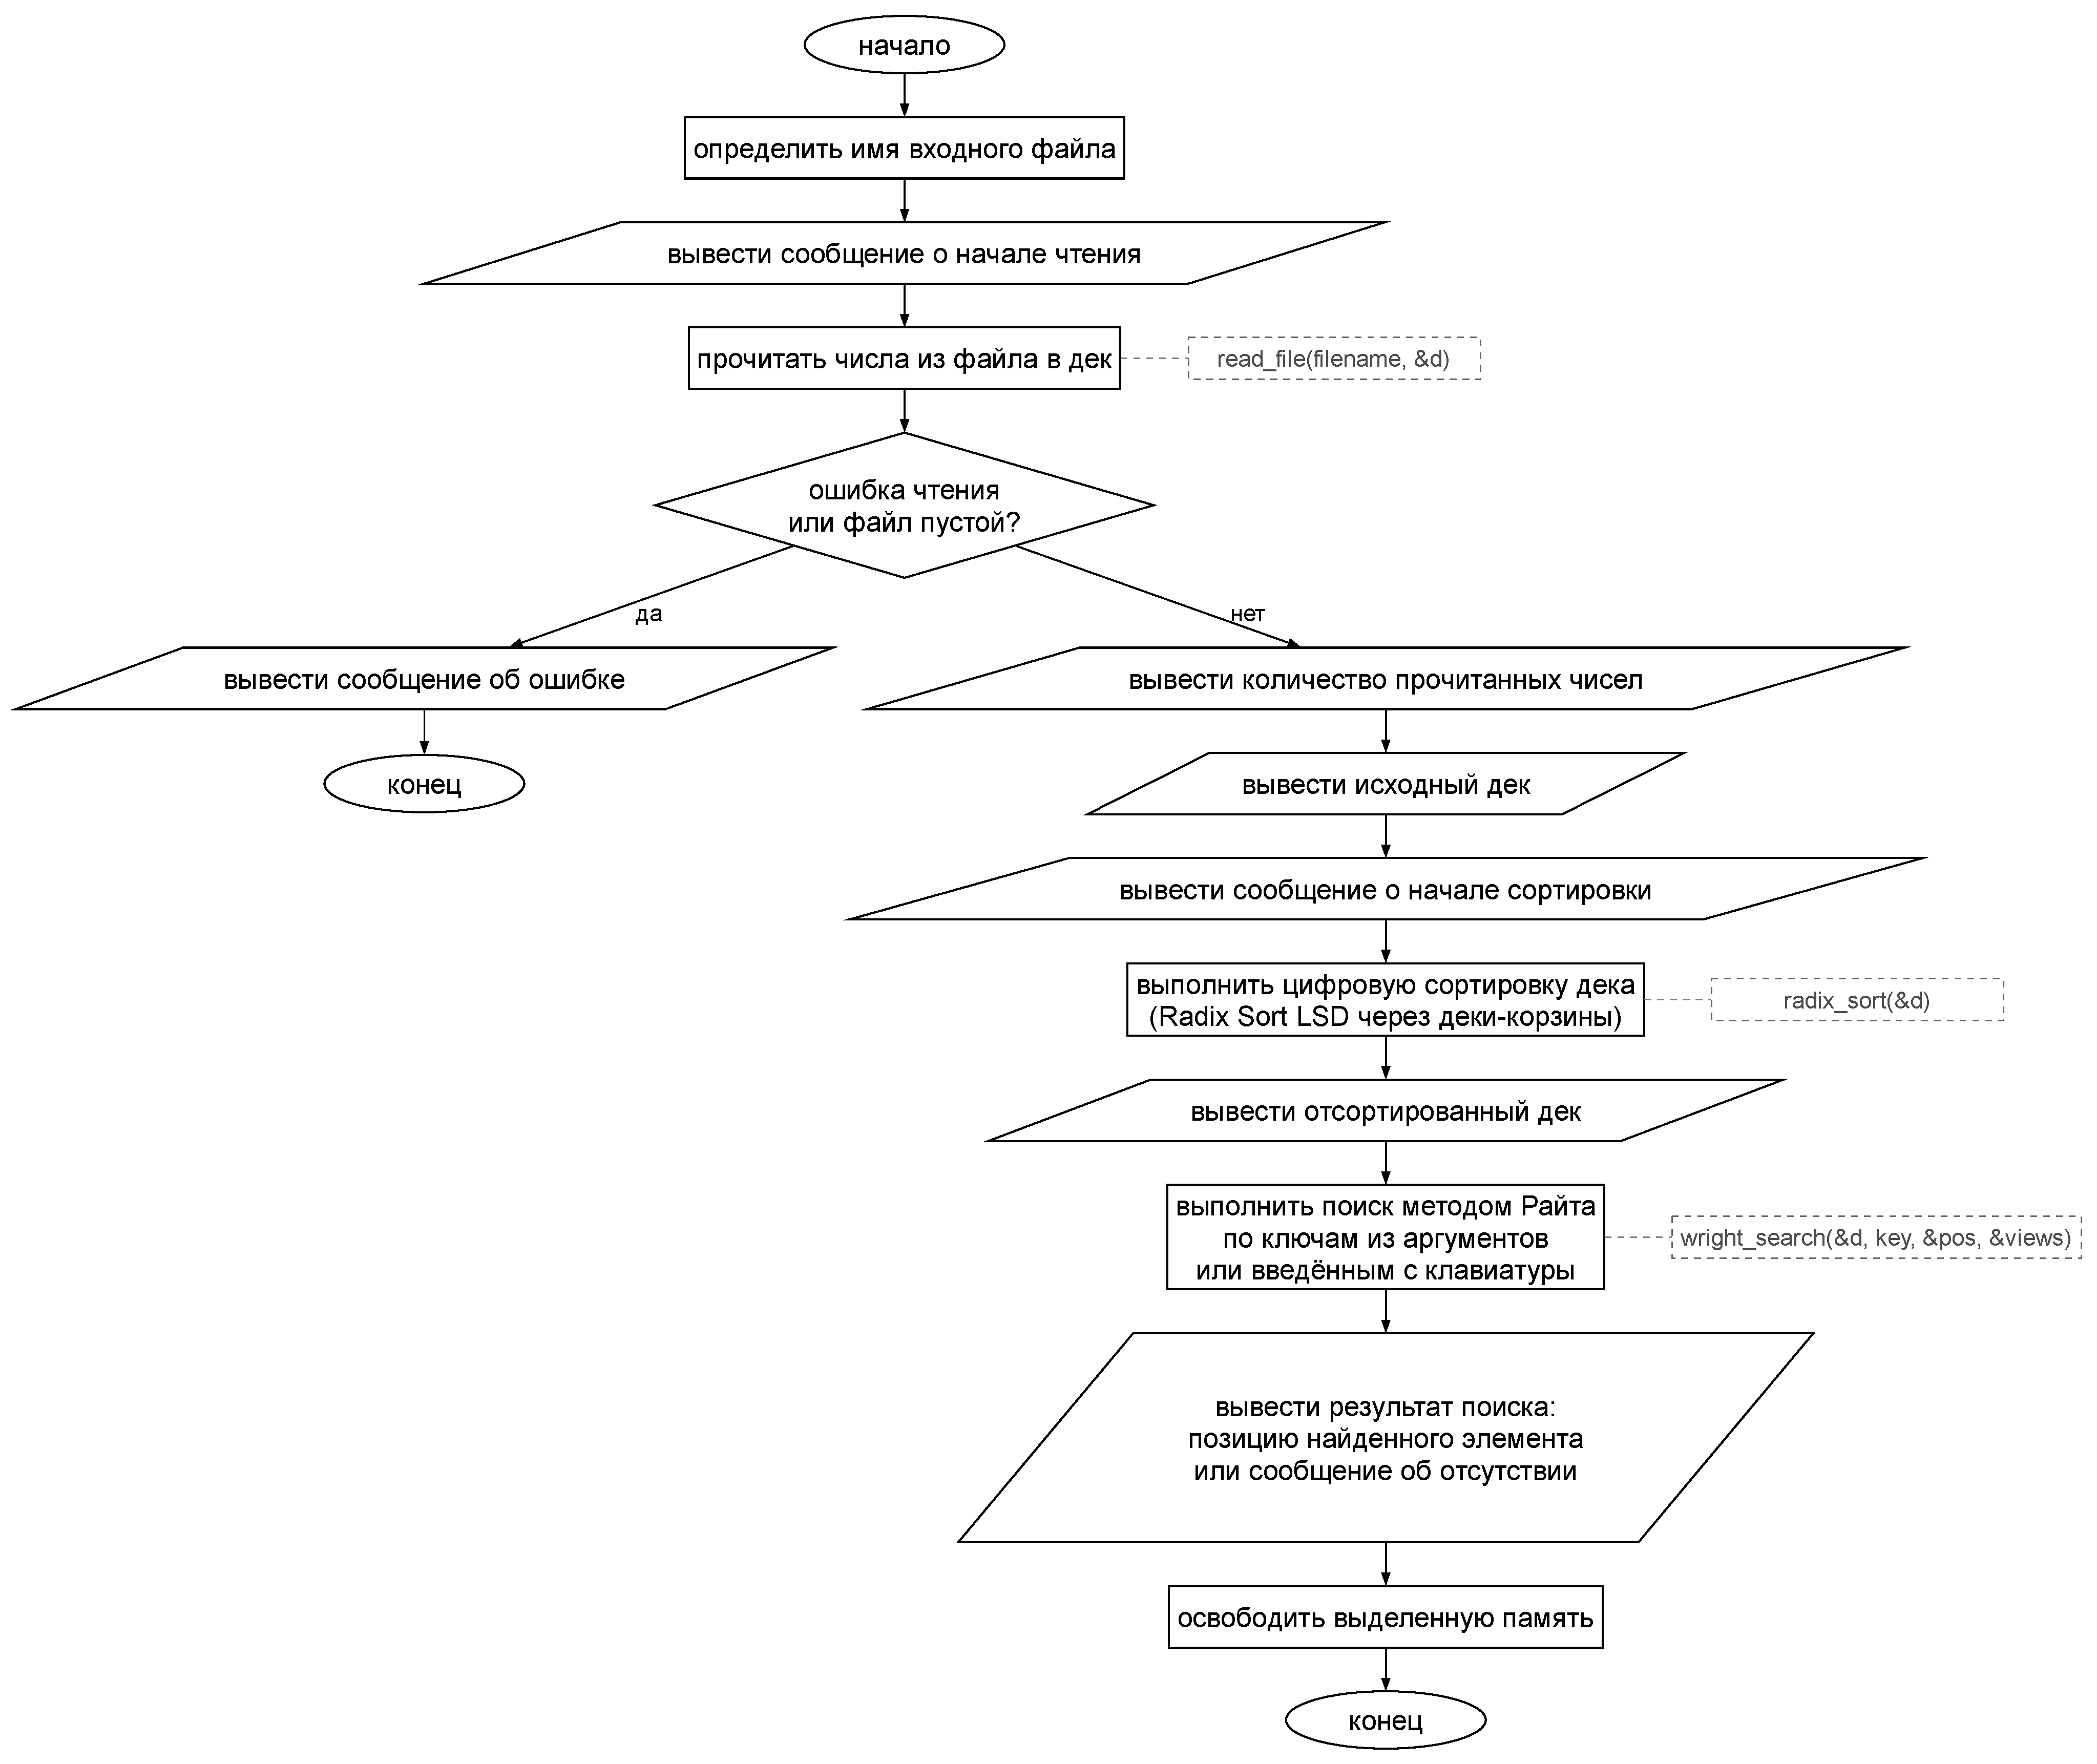
\includegraphics[width=250mm,height=155mm,keepaspectratio]{flowcharts/1_main.pdf}}
\caption{Главная программа (main)}
\end{figure}
\clearpage

\begin{figure}[H]
\centering
\makebox[\linewidth][c]{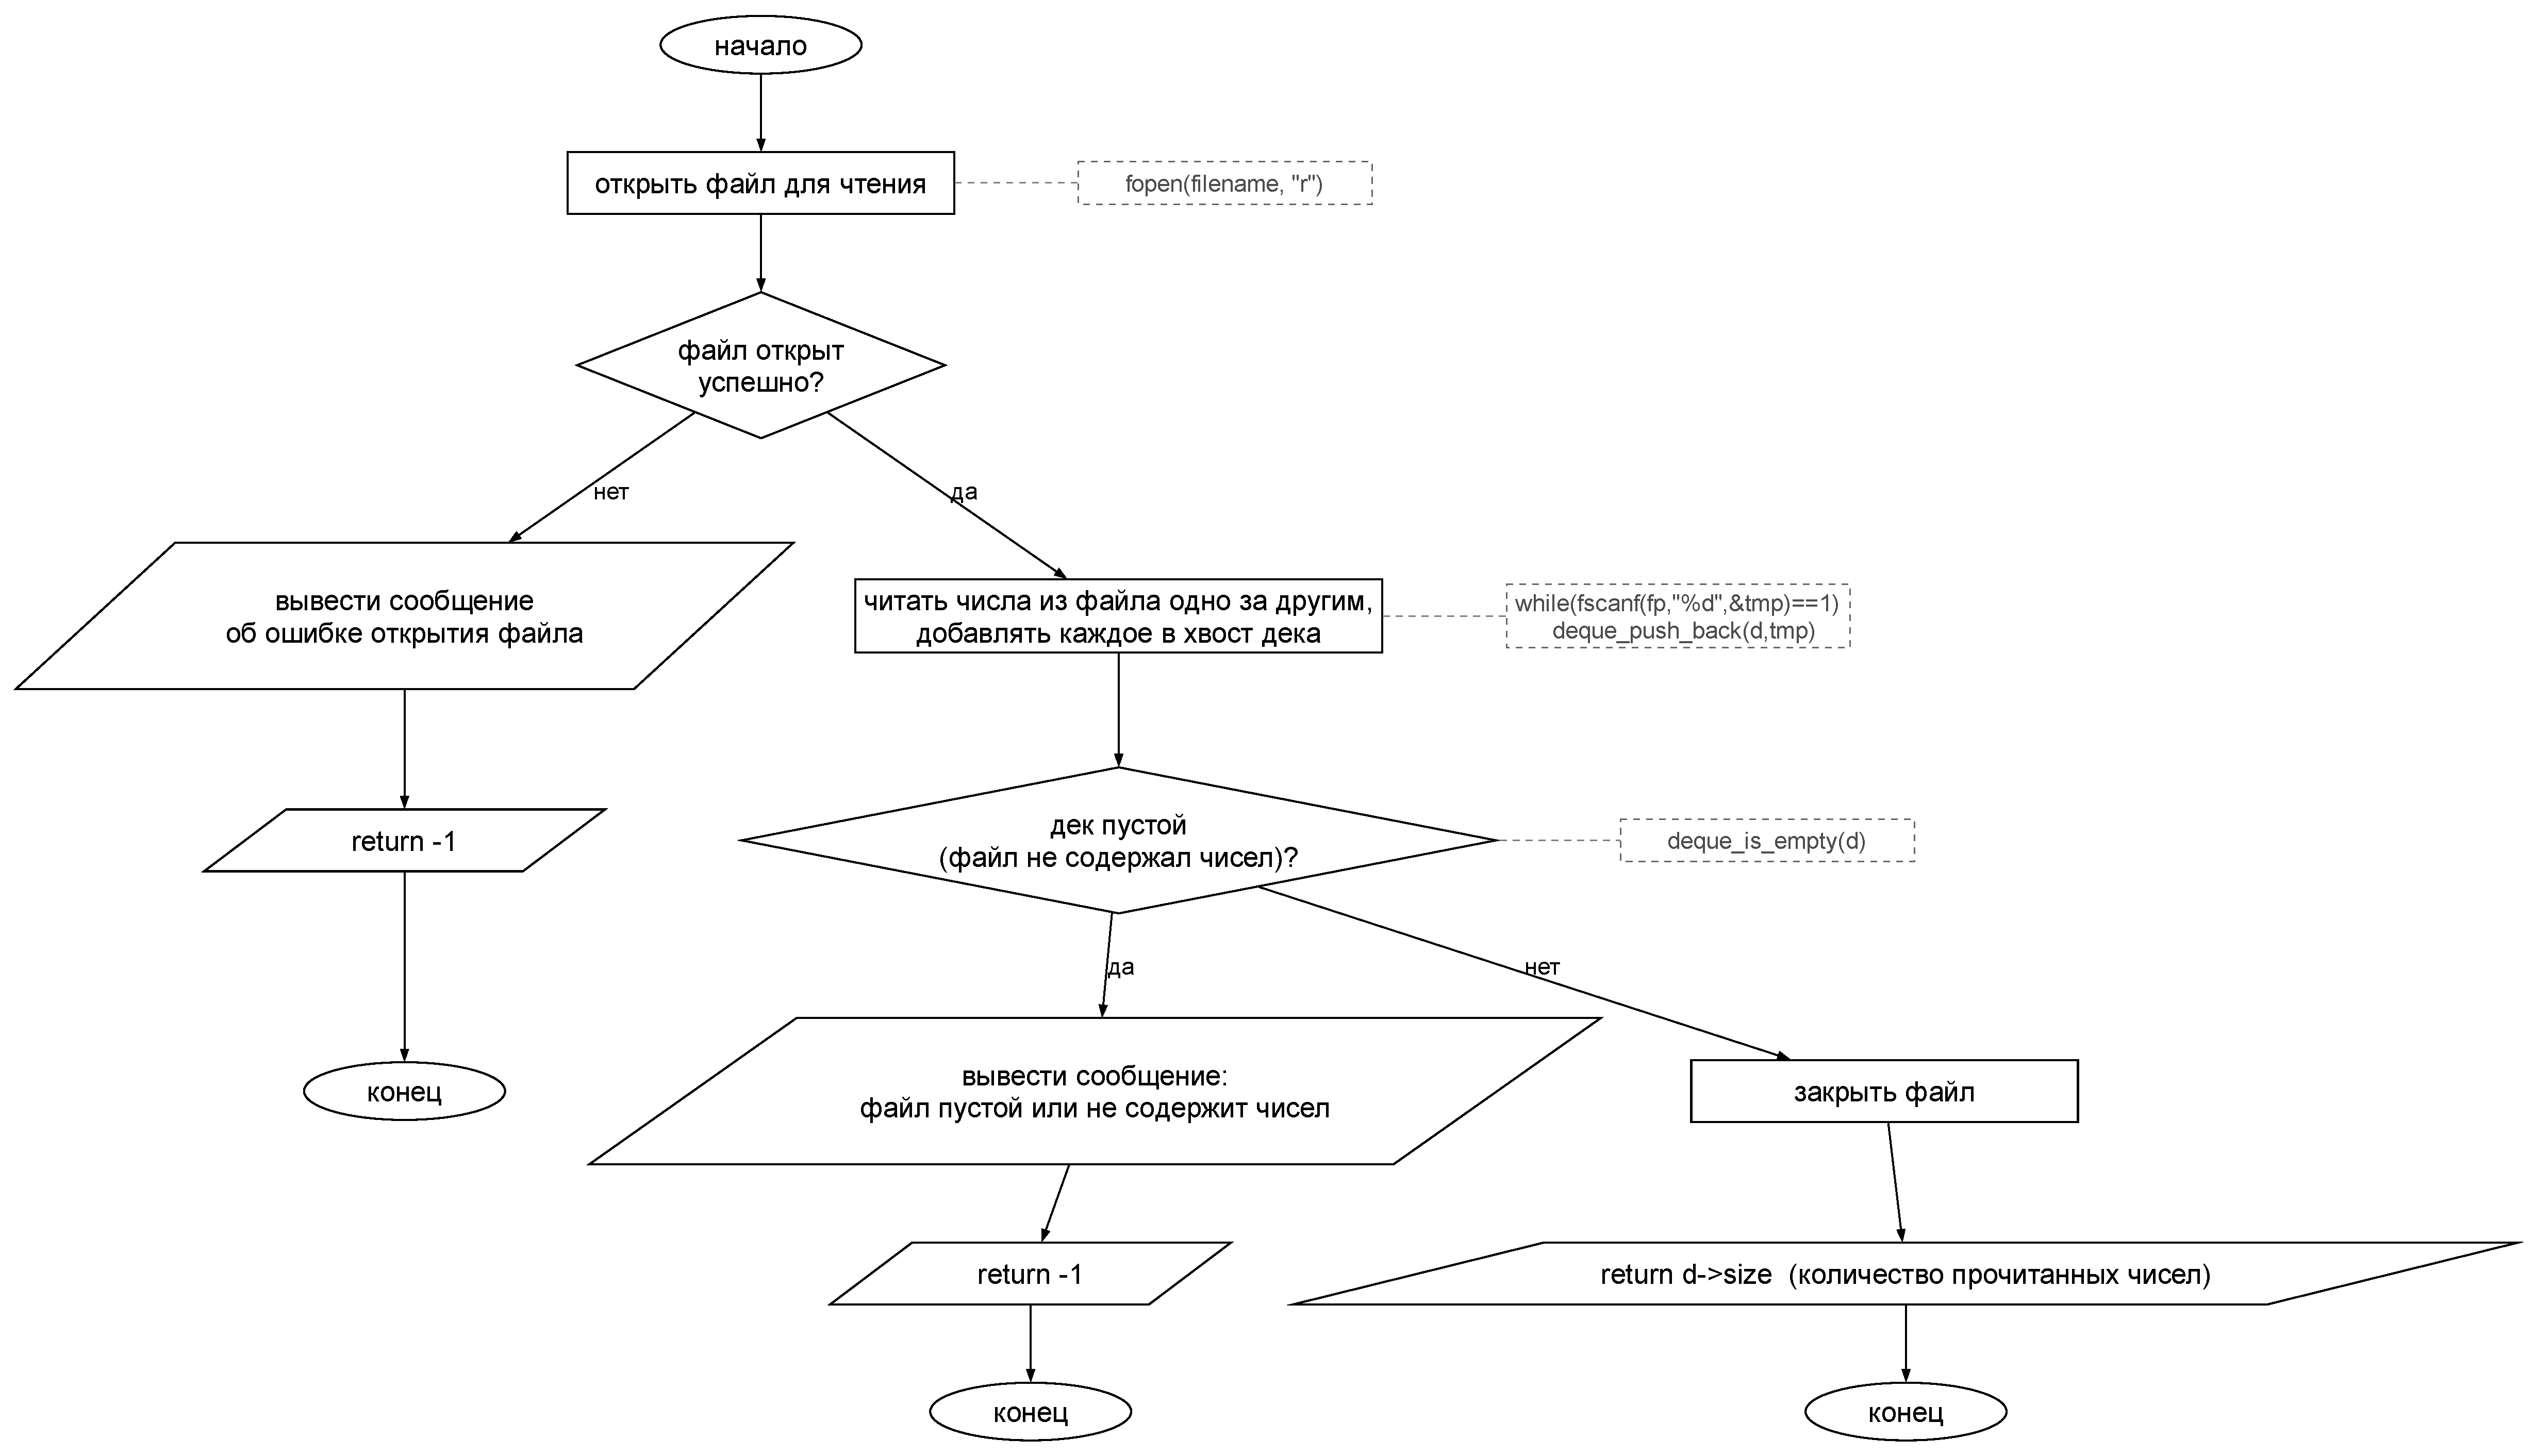
\includegraphics[width=250mm,height=155mm,keepaspectratio]{flowcharts/2_read_file.pdf}}
\caption{Чтение из файла (read\_file)}
\end{figure}
\clearpage

\begin{figure}[H]
\centering
\makebox[\linewidth][c]{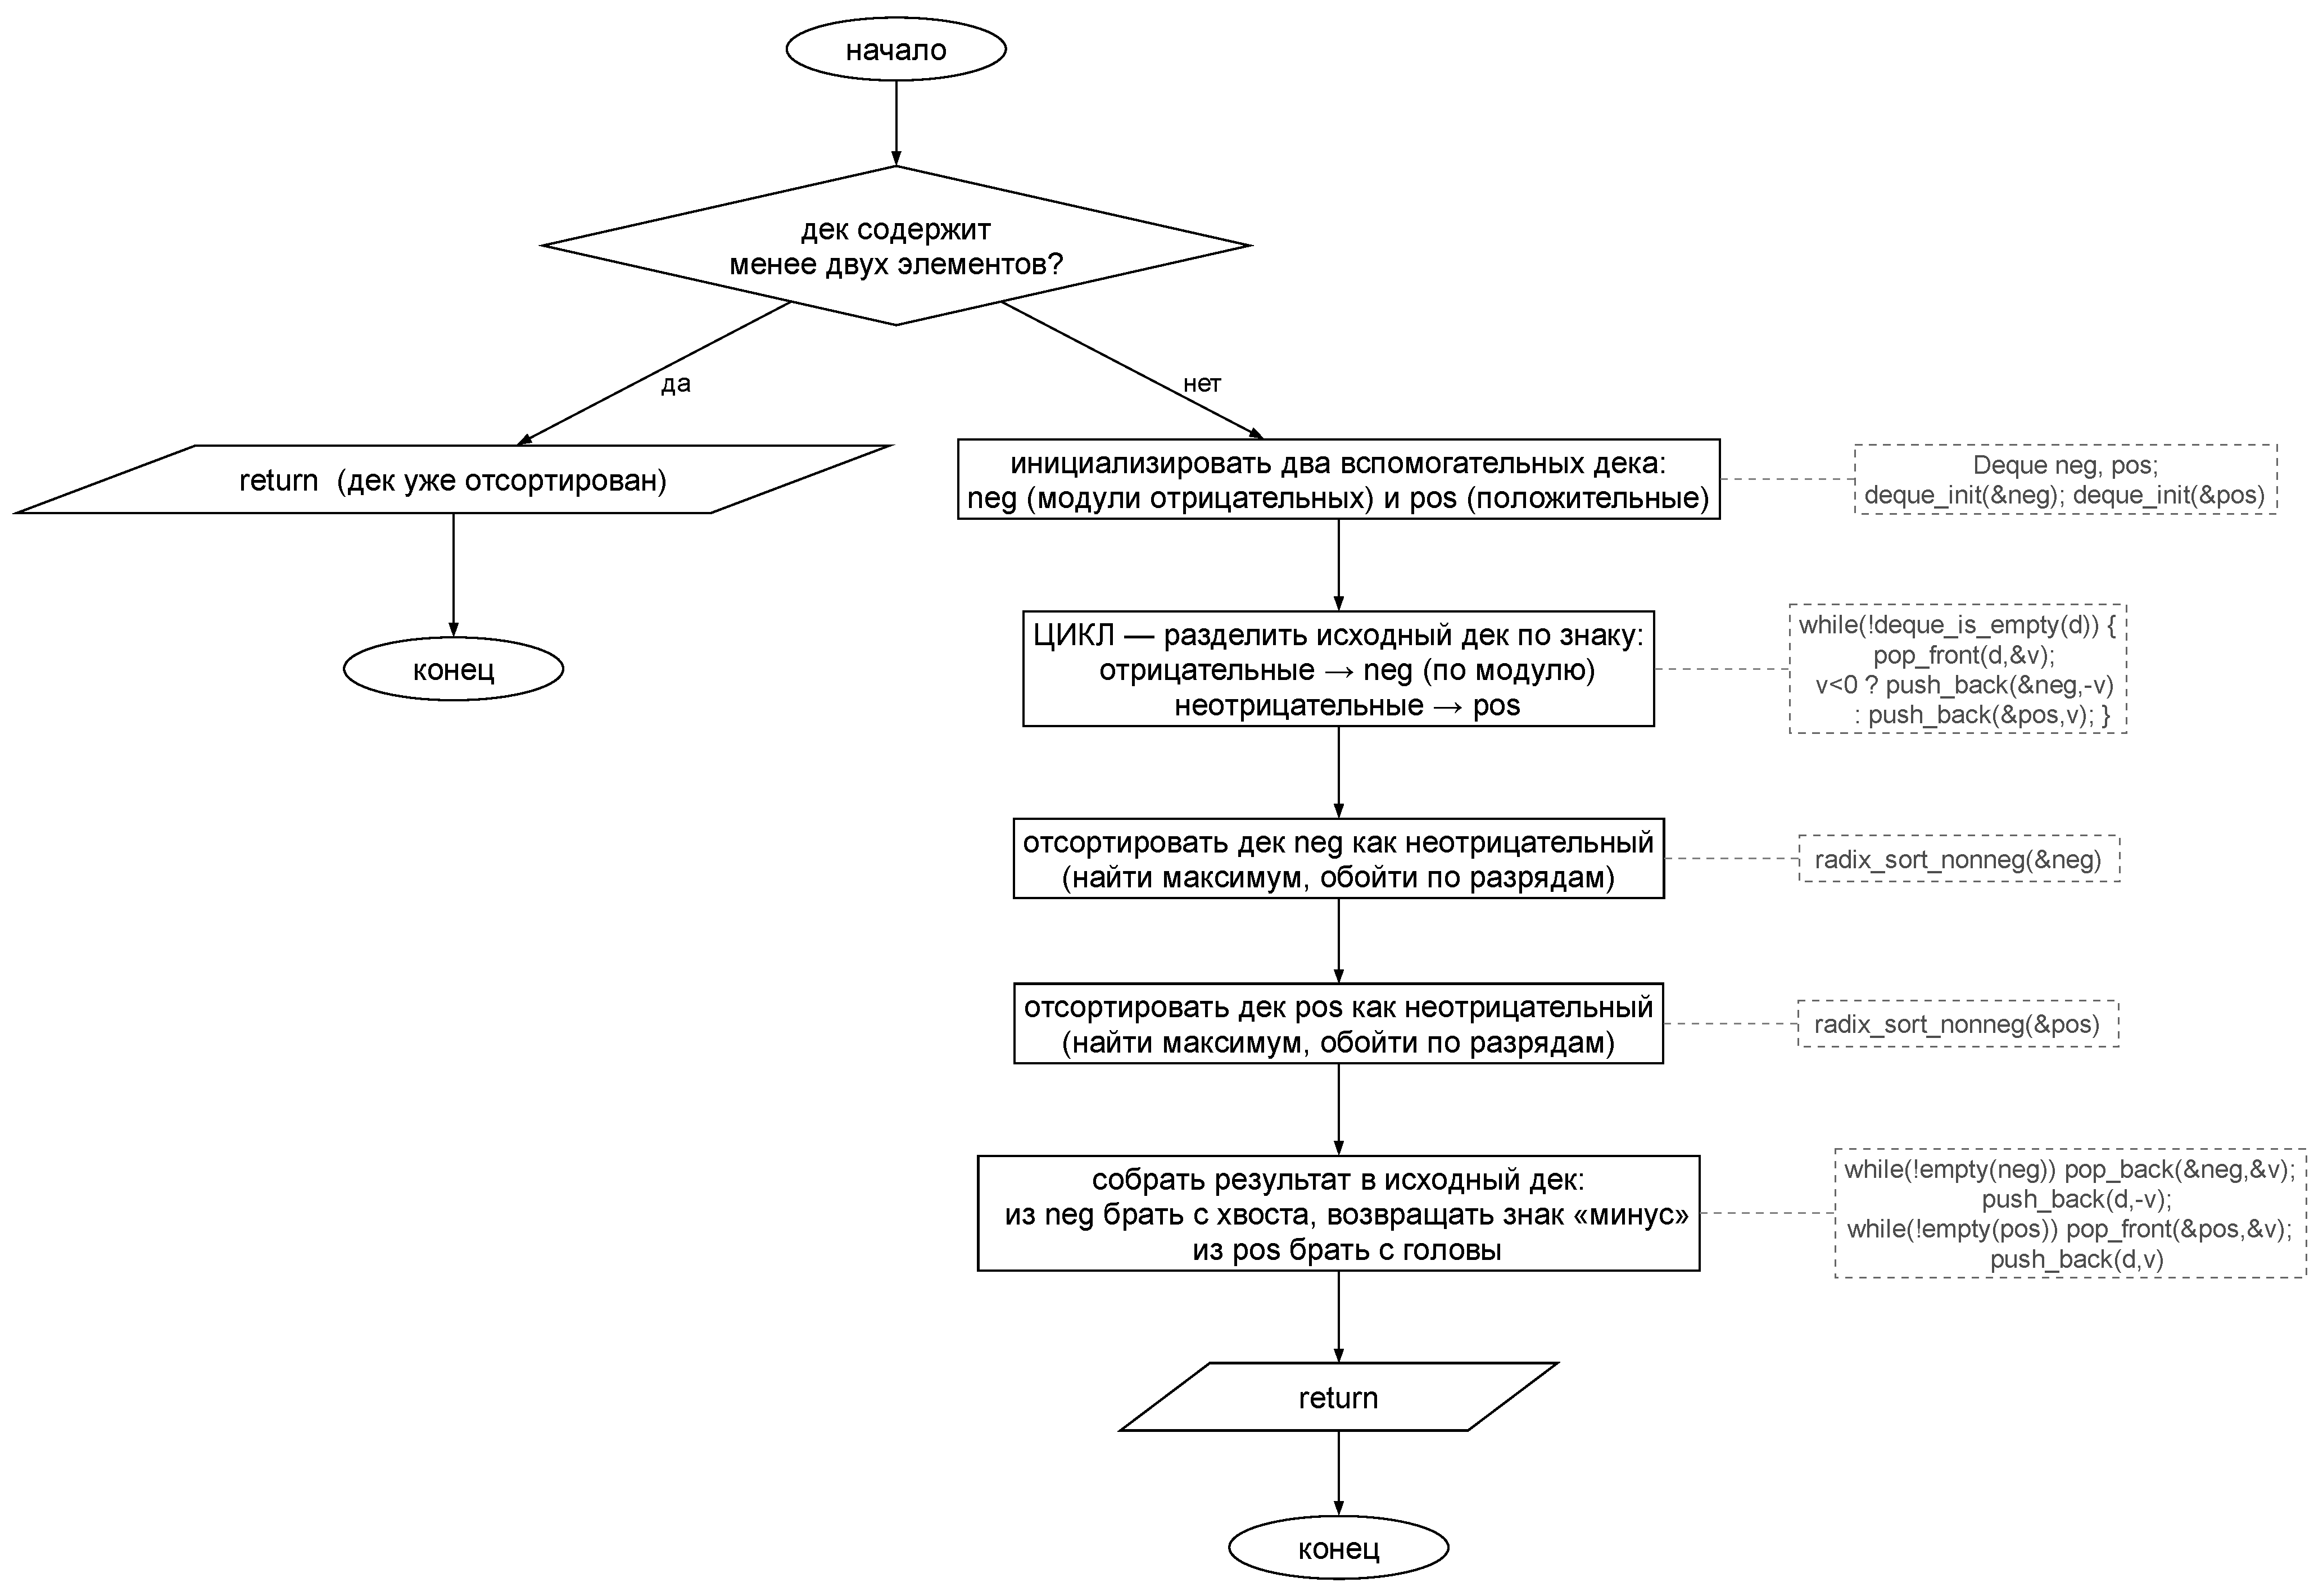
\includegraphics[width=250mm,height=155mm,keepaspectratio]{flowcharts/3_radix_sort.pdf}}
\caption{Цифровая сортировка (radix\_sort)}
\end{figure}

\end{landscape}

\begin{figure}[H]
\centering
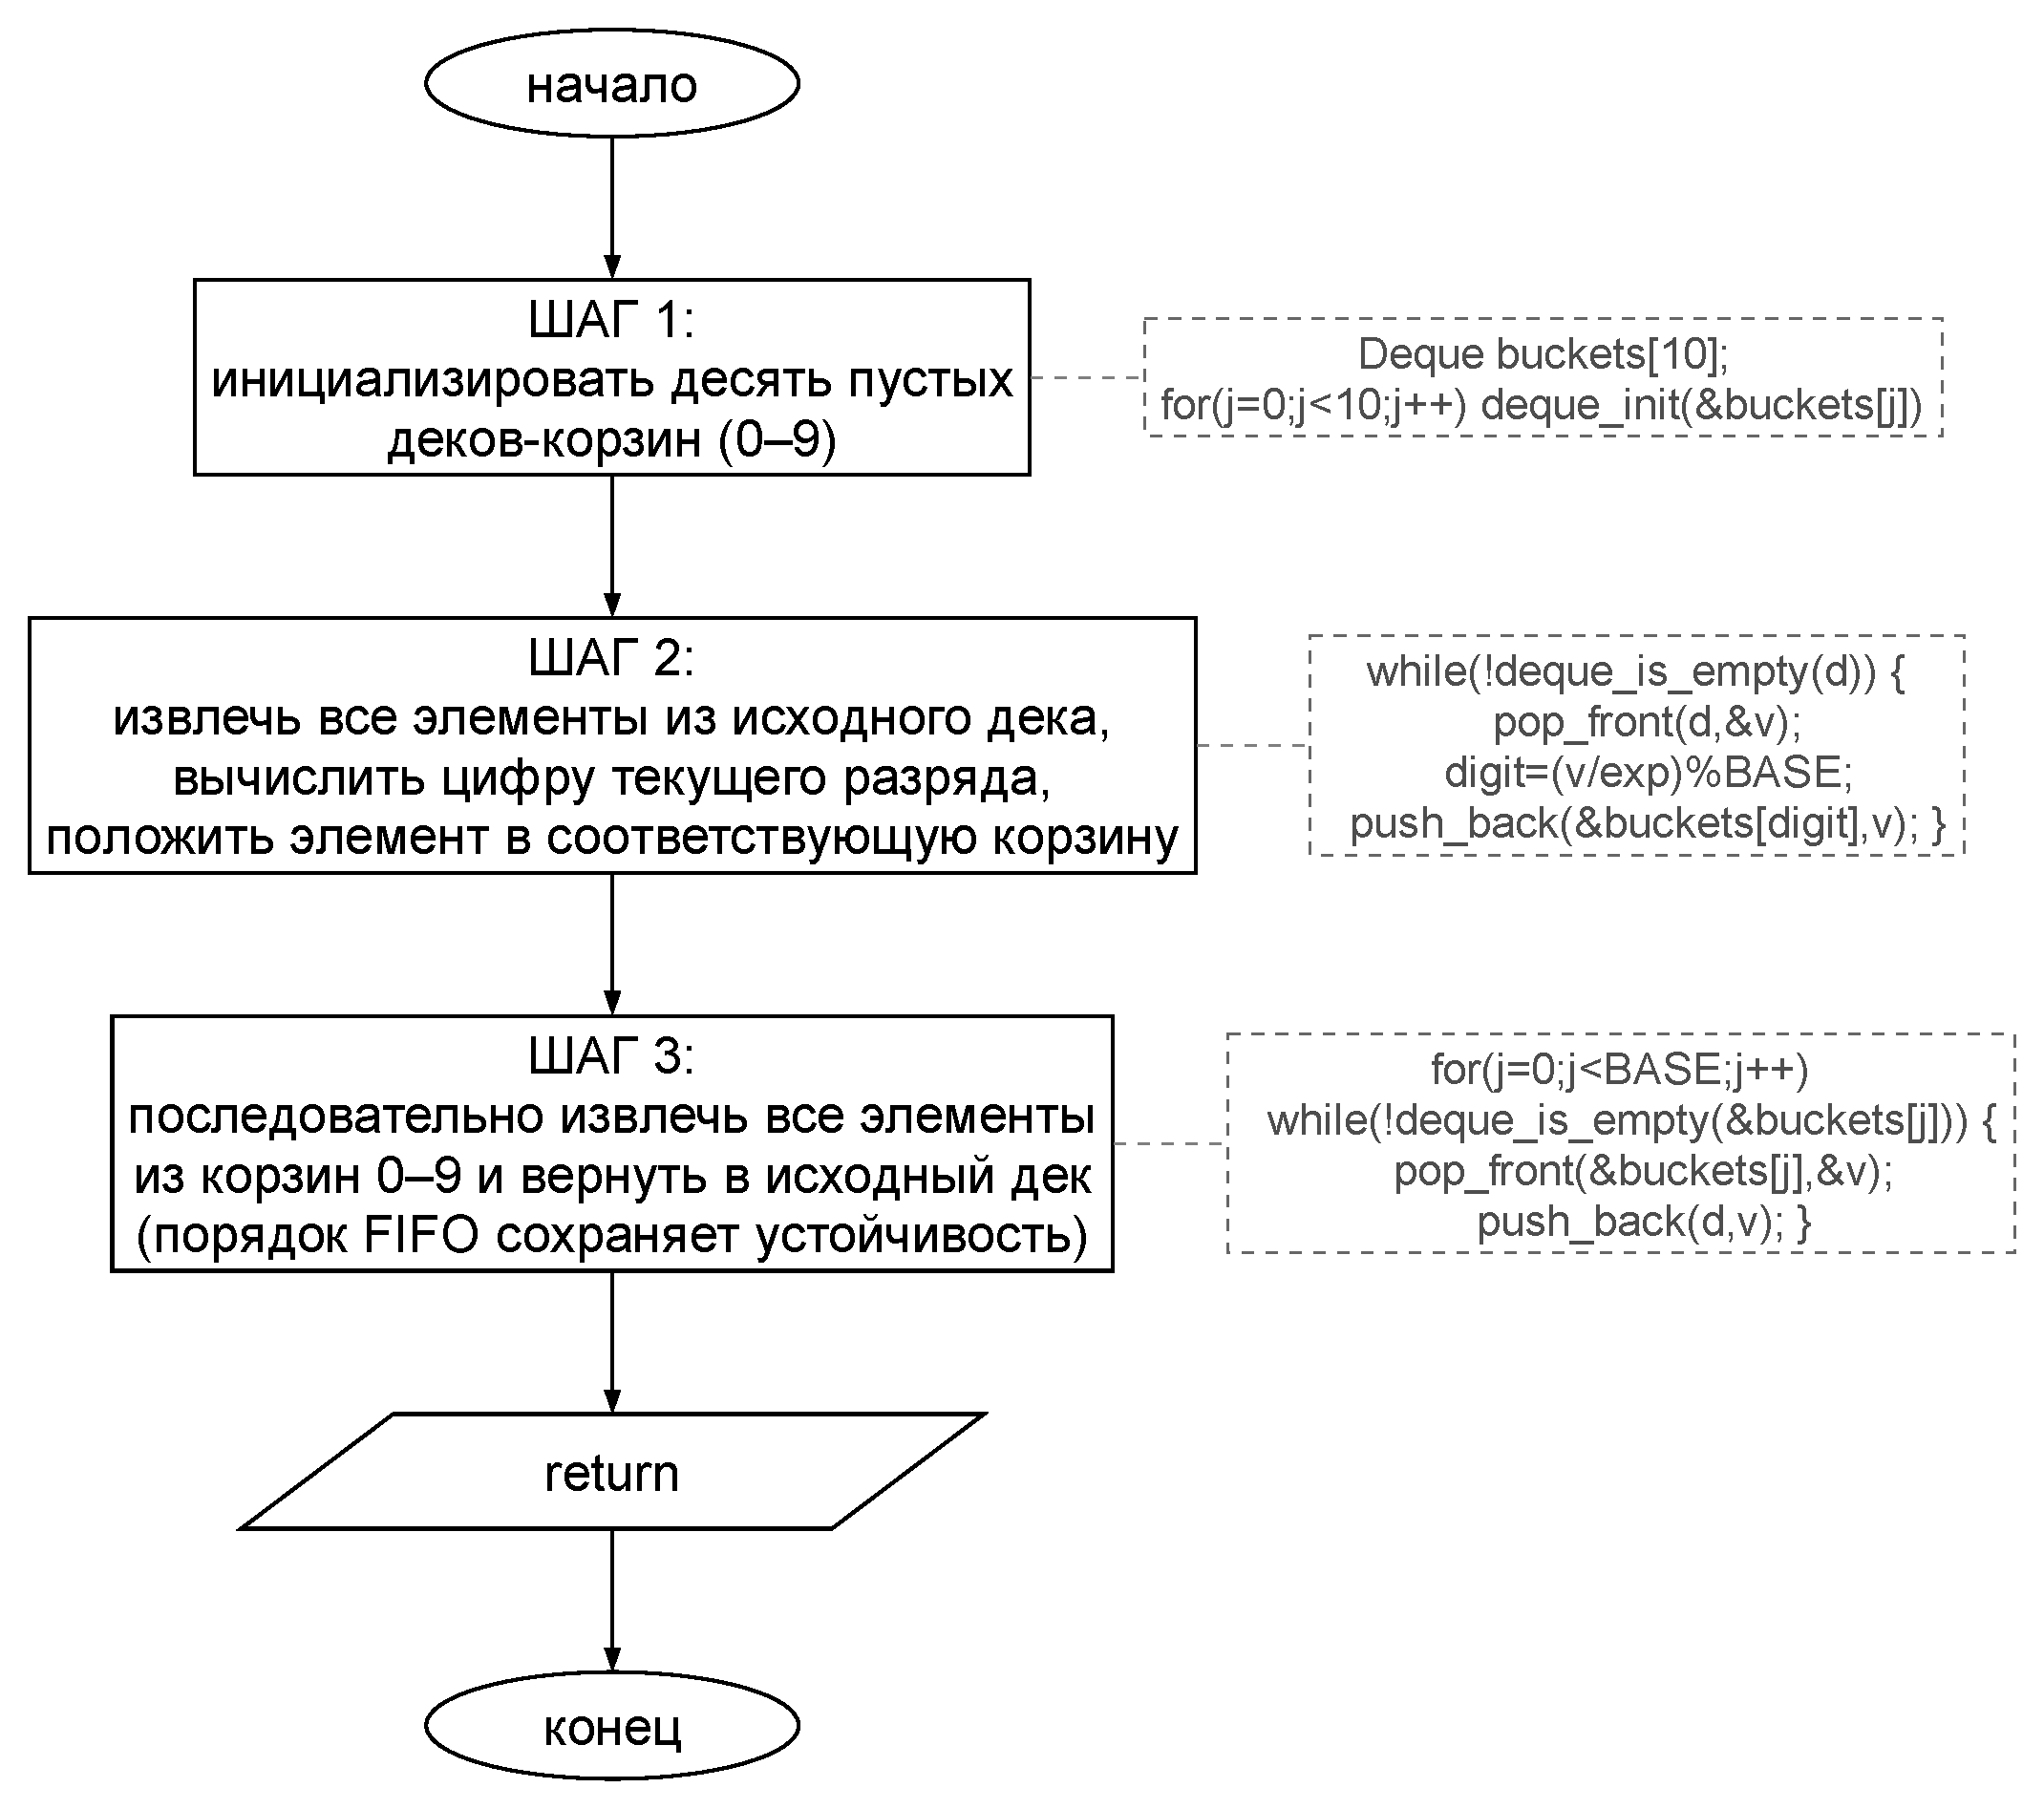
\includegraphics[width=\textwidth]{flowcharts/4_counting_sort_deque.pdf}
\caption{Сортировка по разряду через деки (counting\_sort\_by\_deque)}
\end{figure}

\begin{landscape}

\begin{figure}[H]
\centering
\makebox[\linewidth][c]{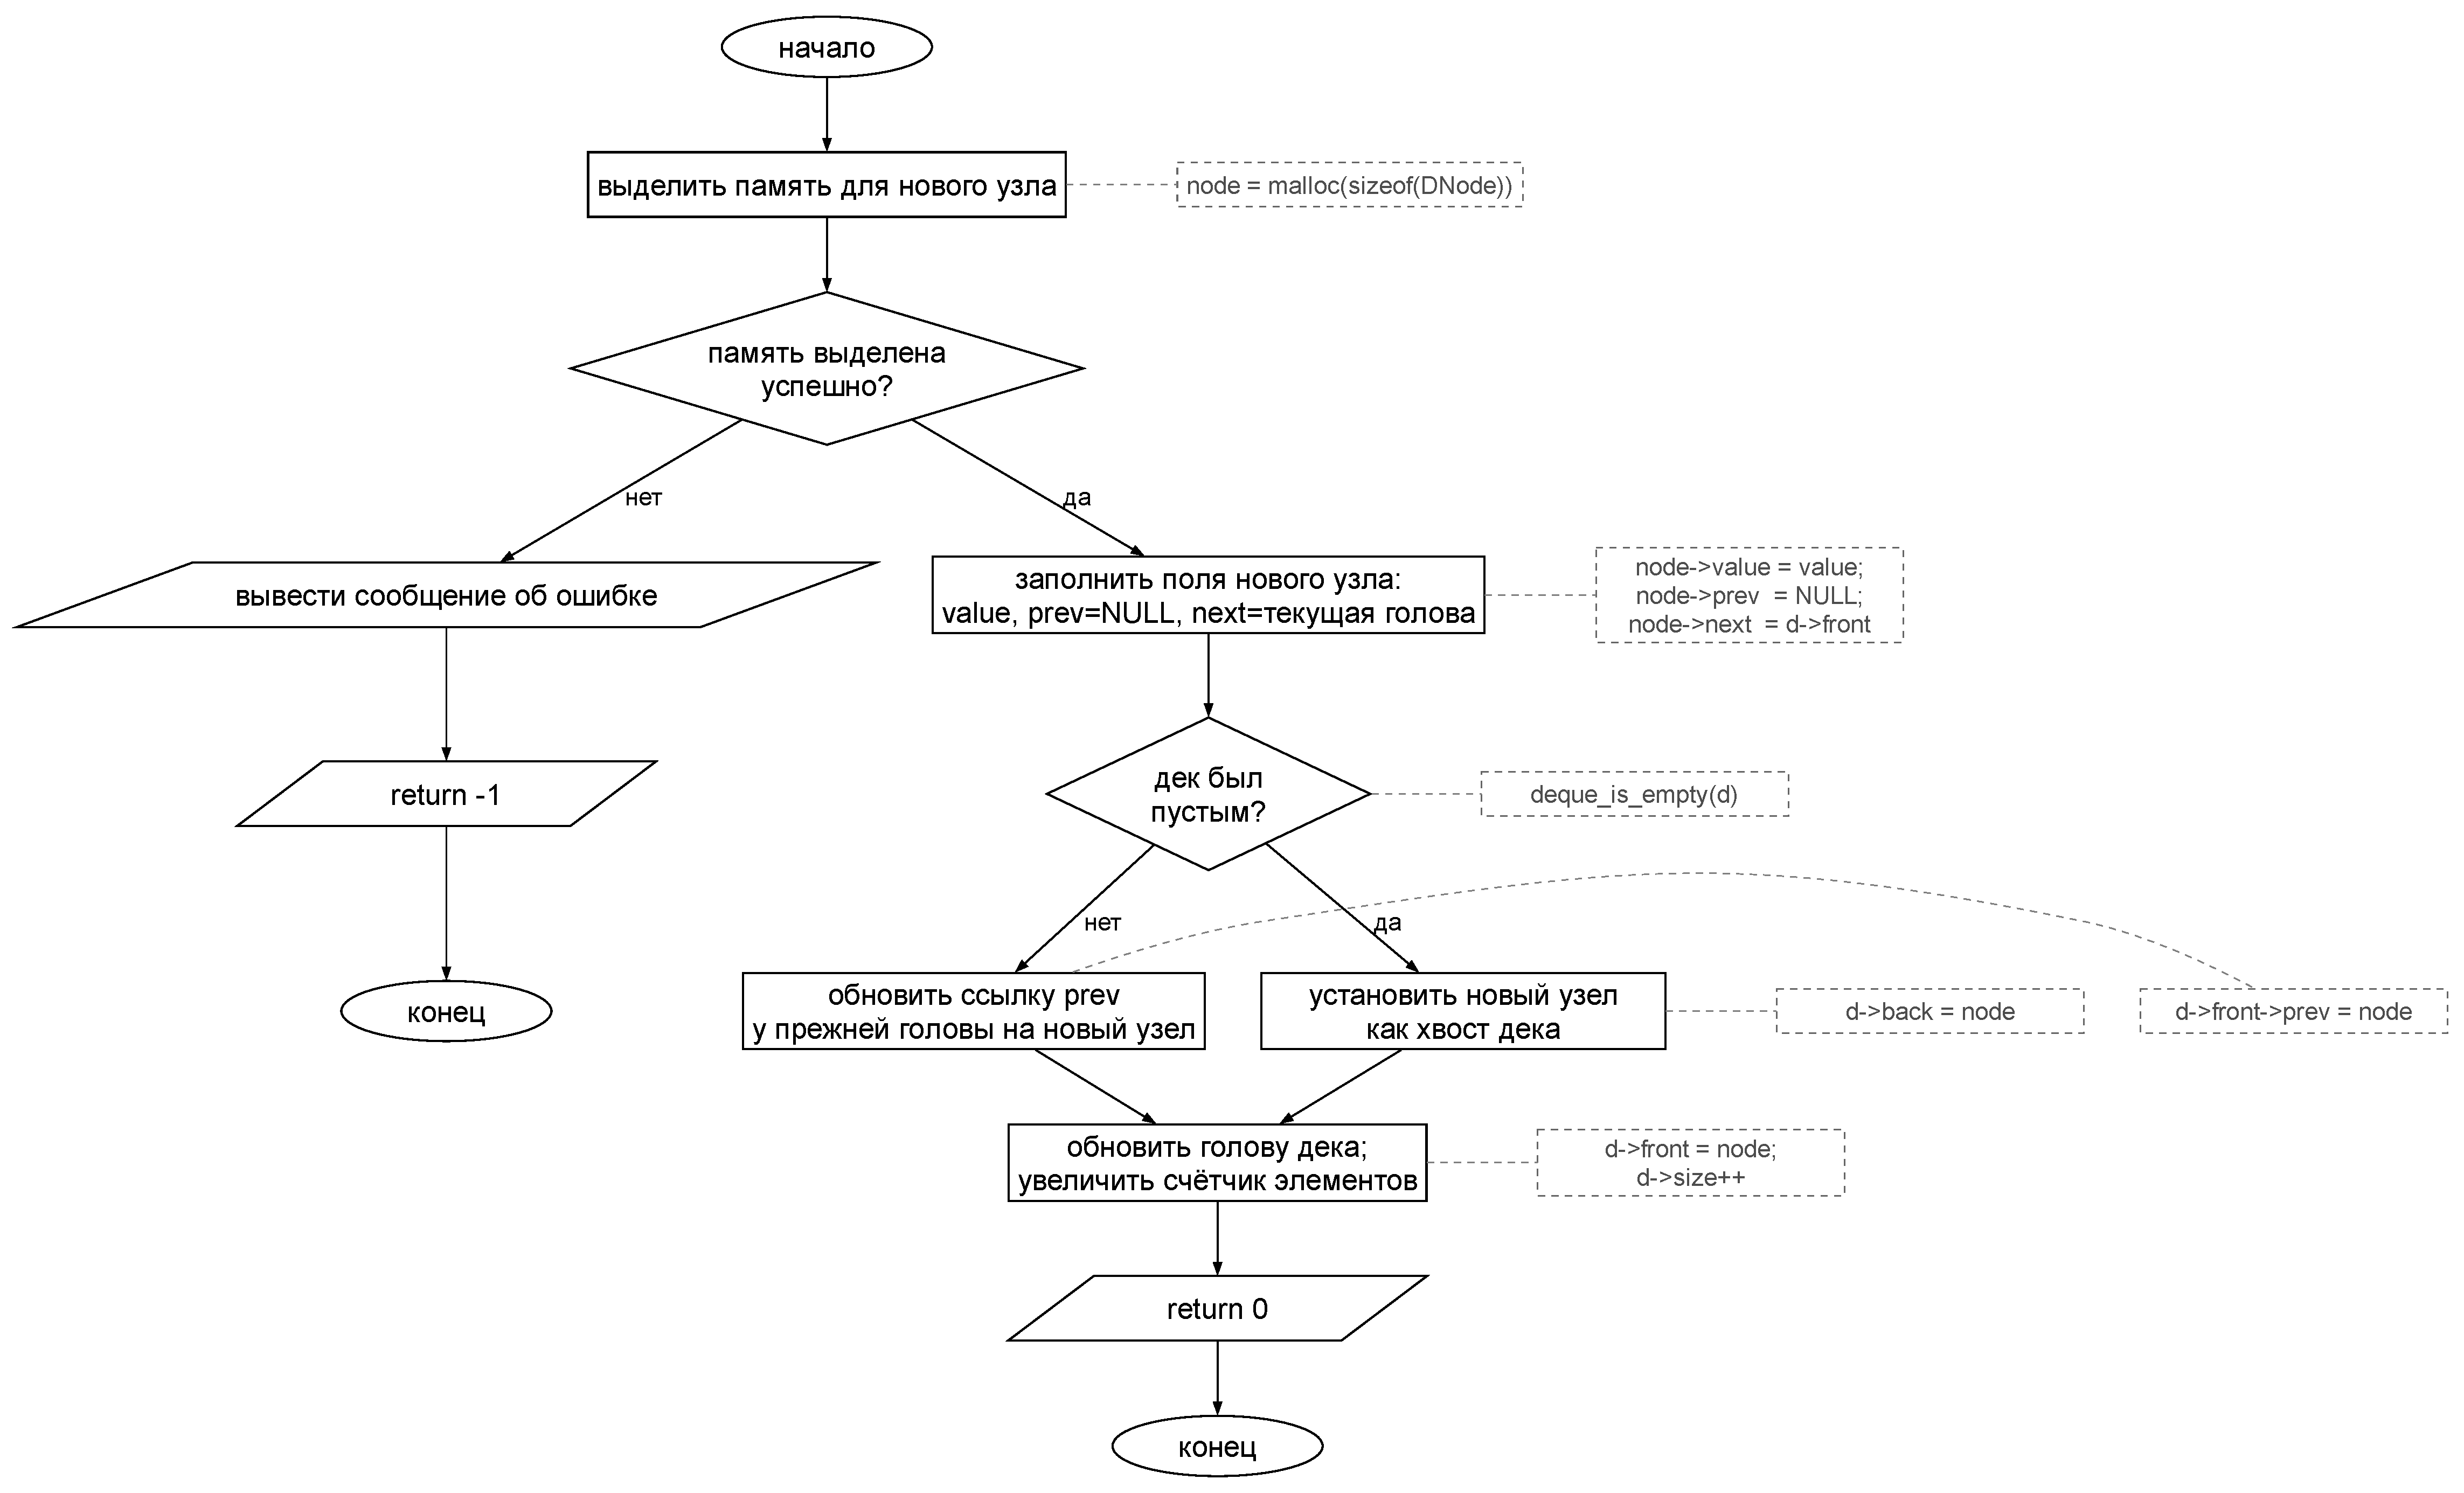
\includegraphics[width=250mm,height=155mm,keepaspectratio]{flowcharts/5a_push_front.pdf}}
\caption{Добавление в голову дека (push\_front)}
\end{figure}
\clearpage

\begin{figure}[H]
\centering
\makebox[\linewidth][c]{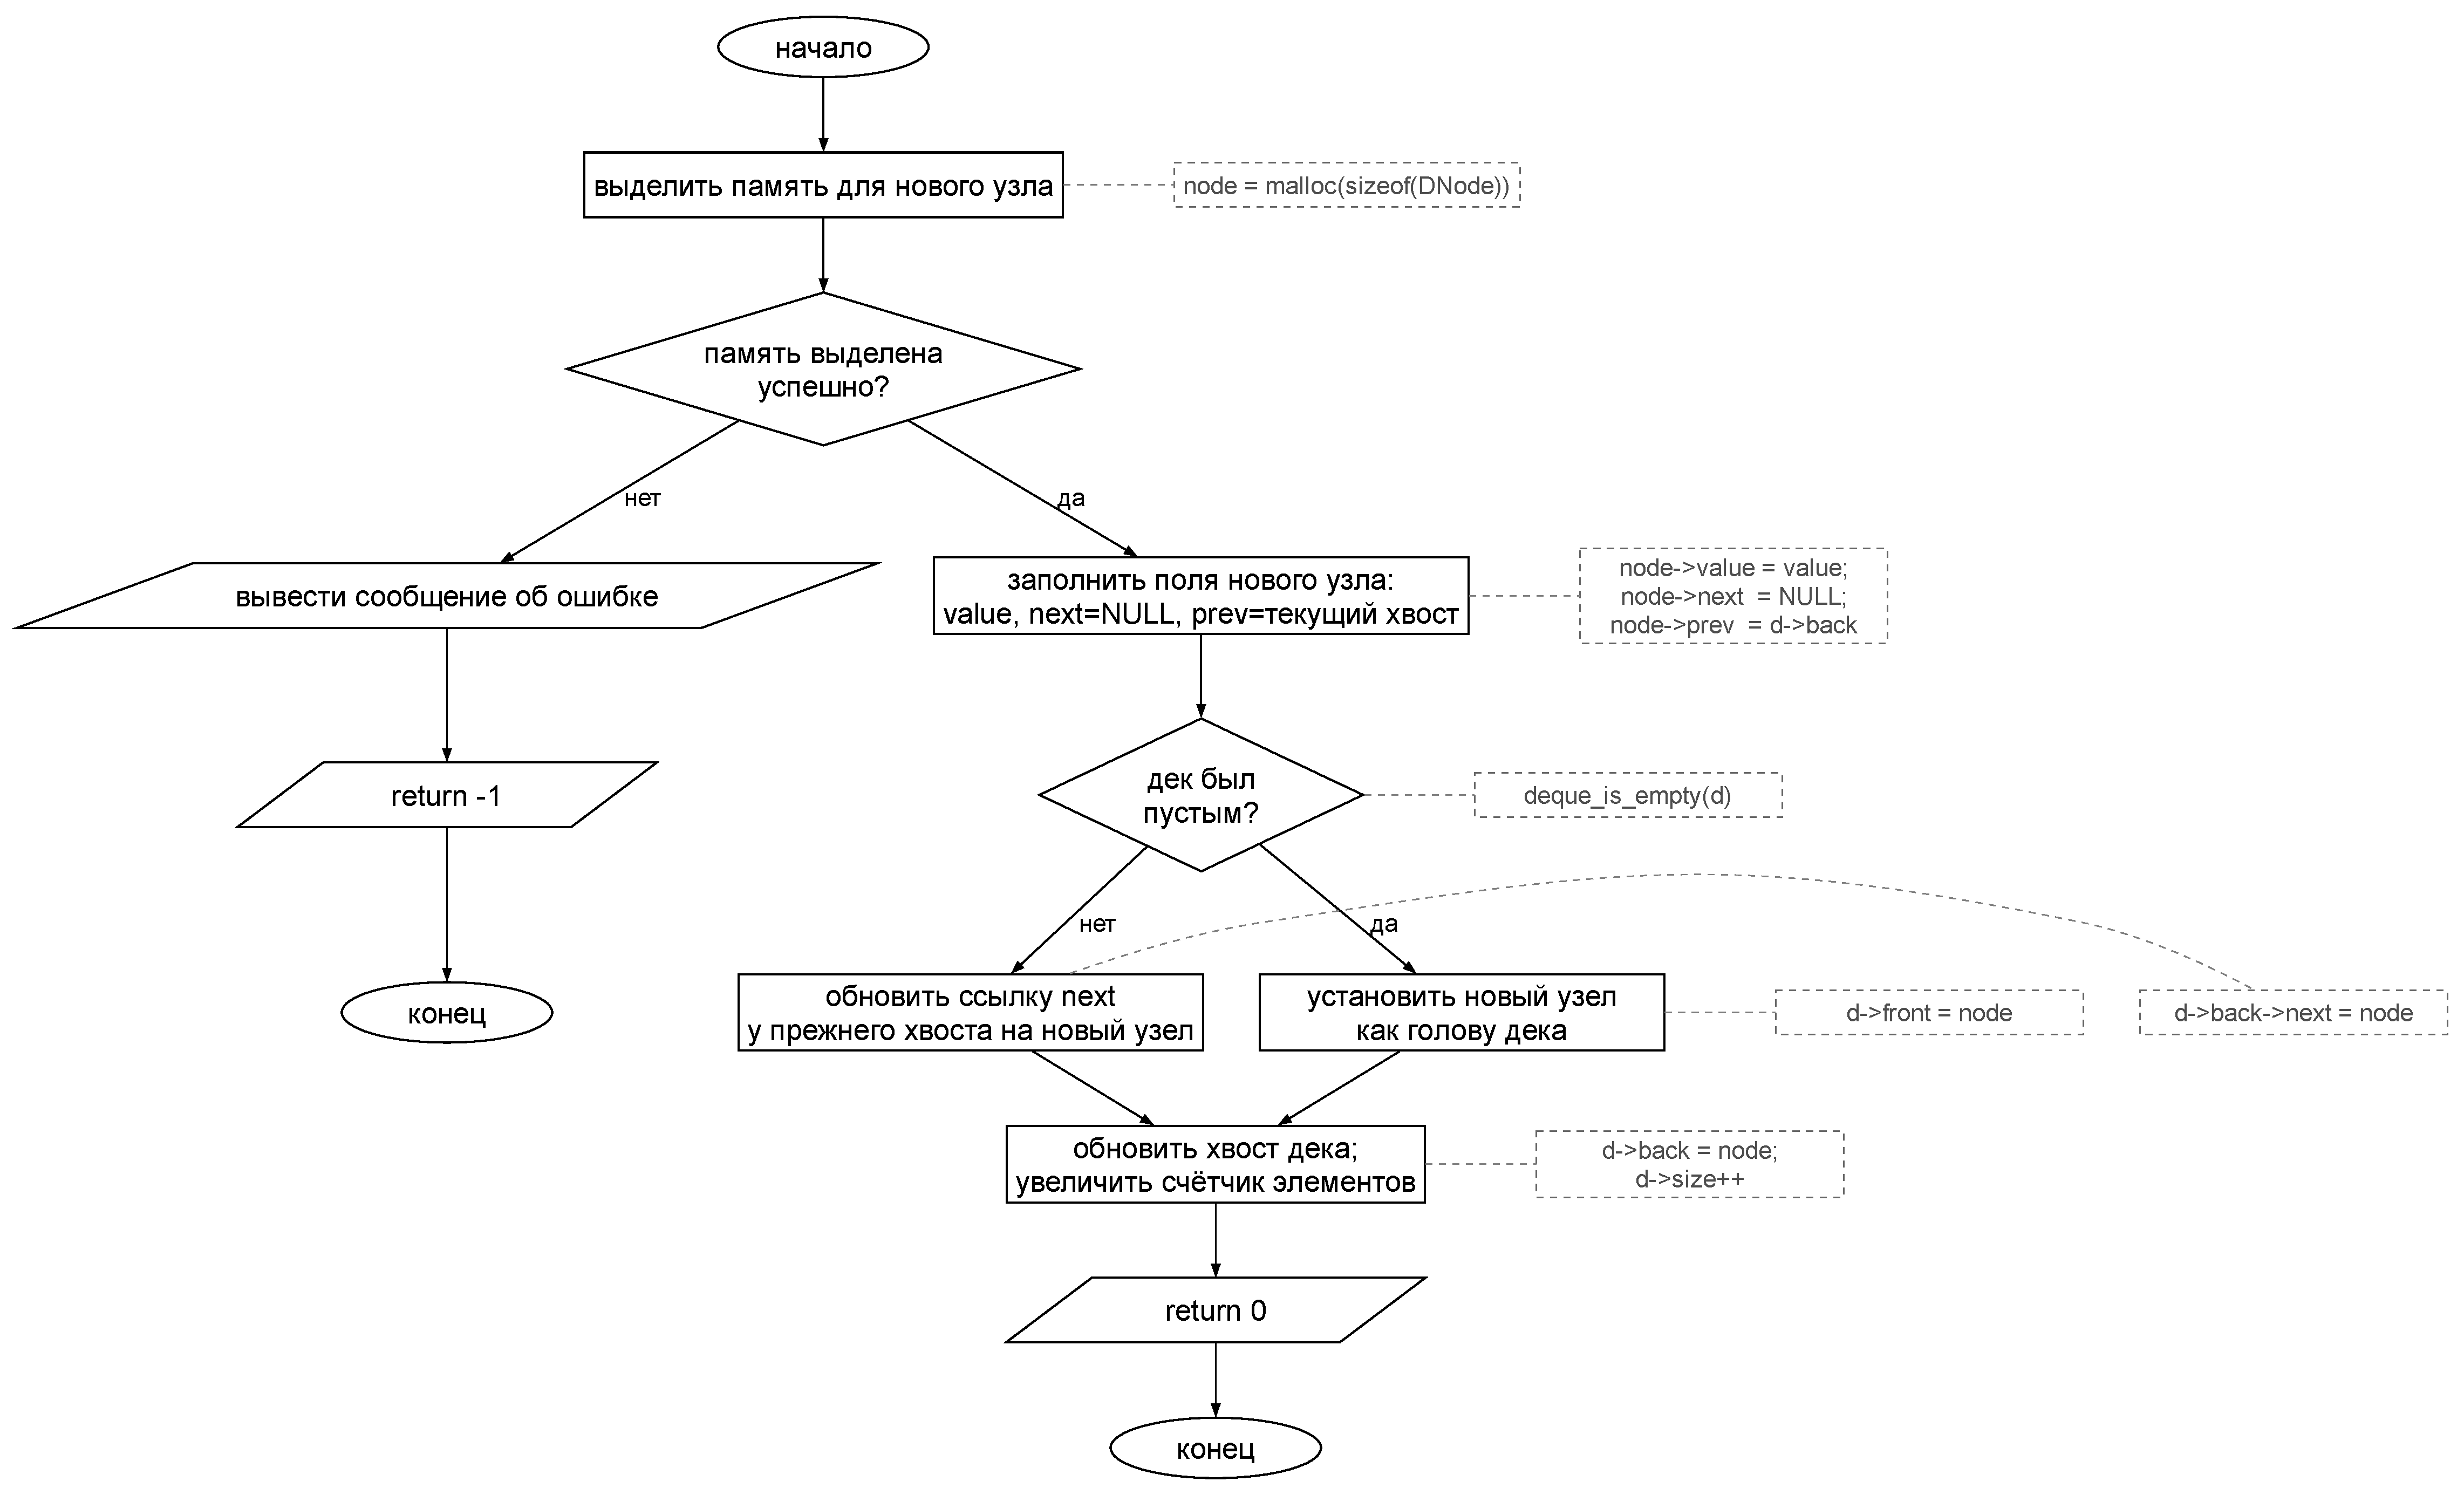
\includegraphics[width=250mm,height=155mm,keepaspectratio]{flowcharts/5b_push_back.pdf}}
\caption{Добавление в хвост дека (push\_back)}
\end{figure}
\clearpage

\begin{figure}[H]
\centering
\makebox[\linewidth][c]{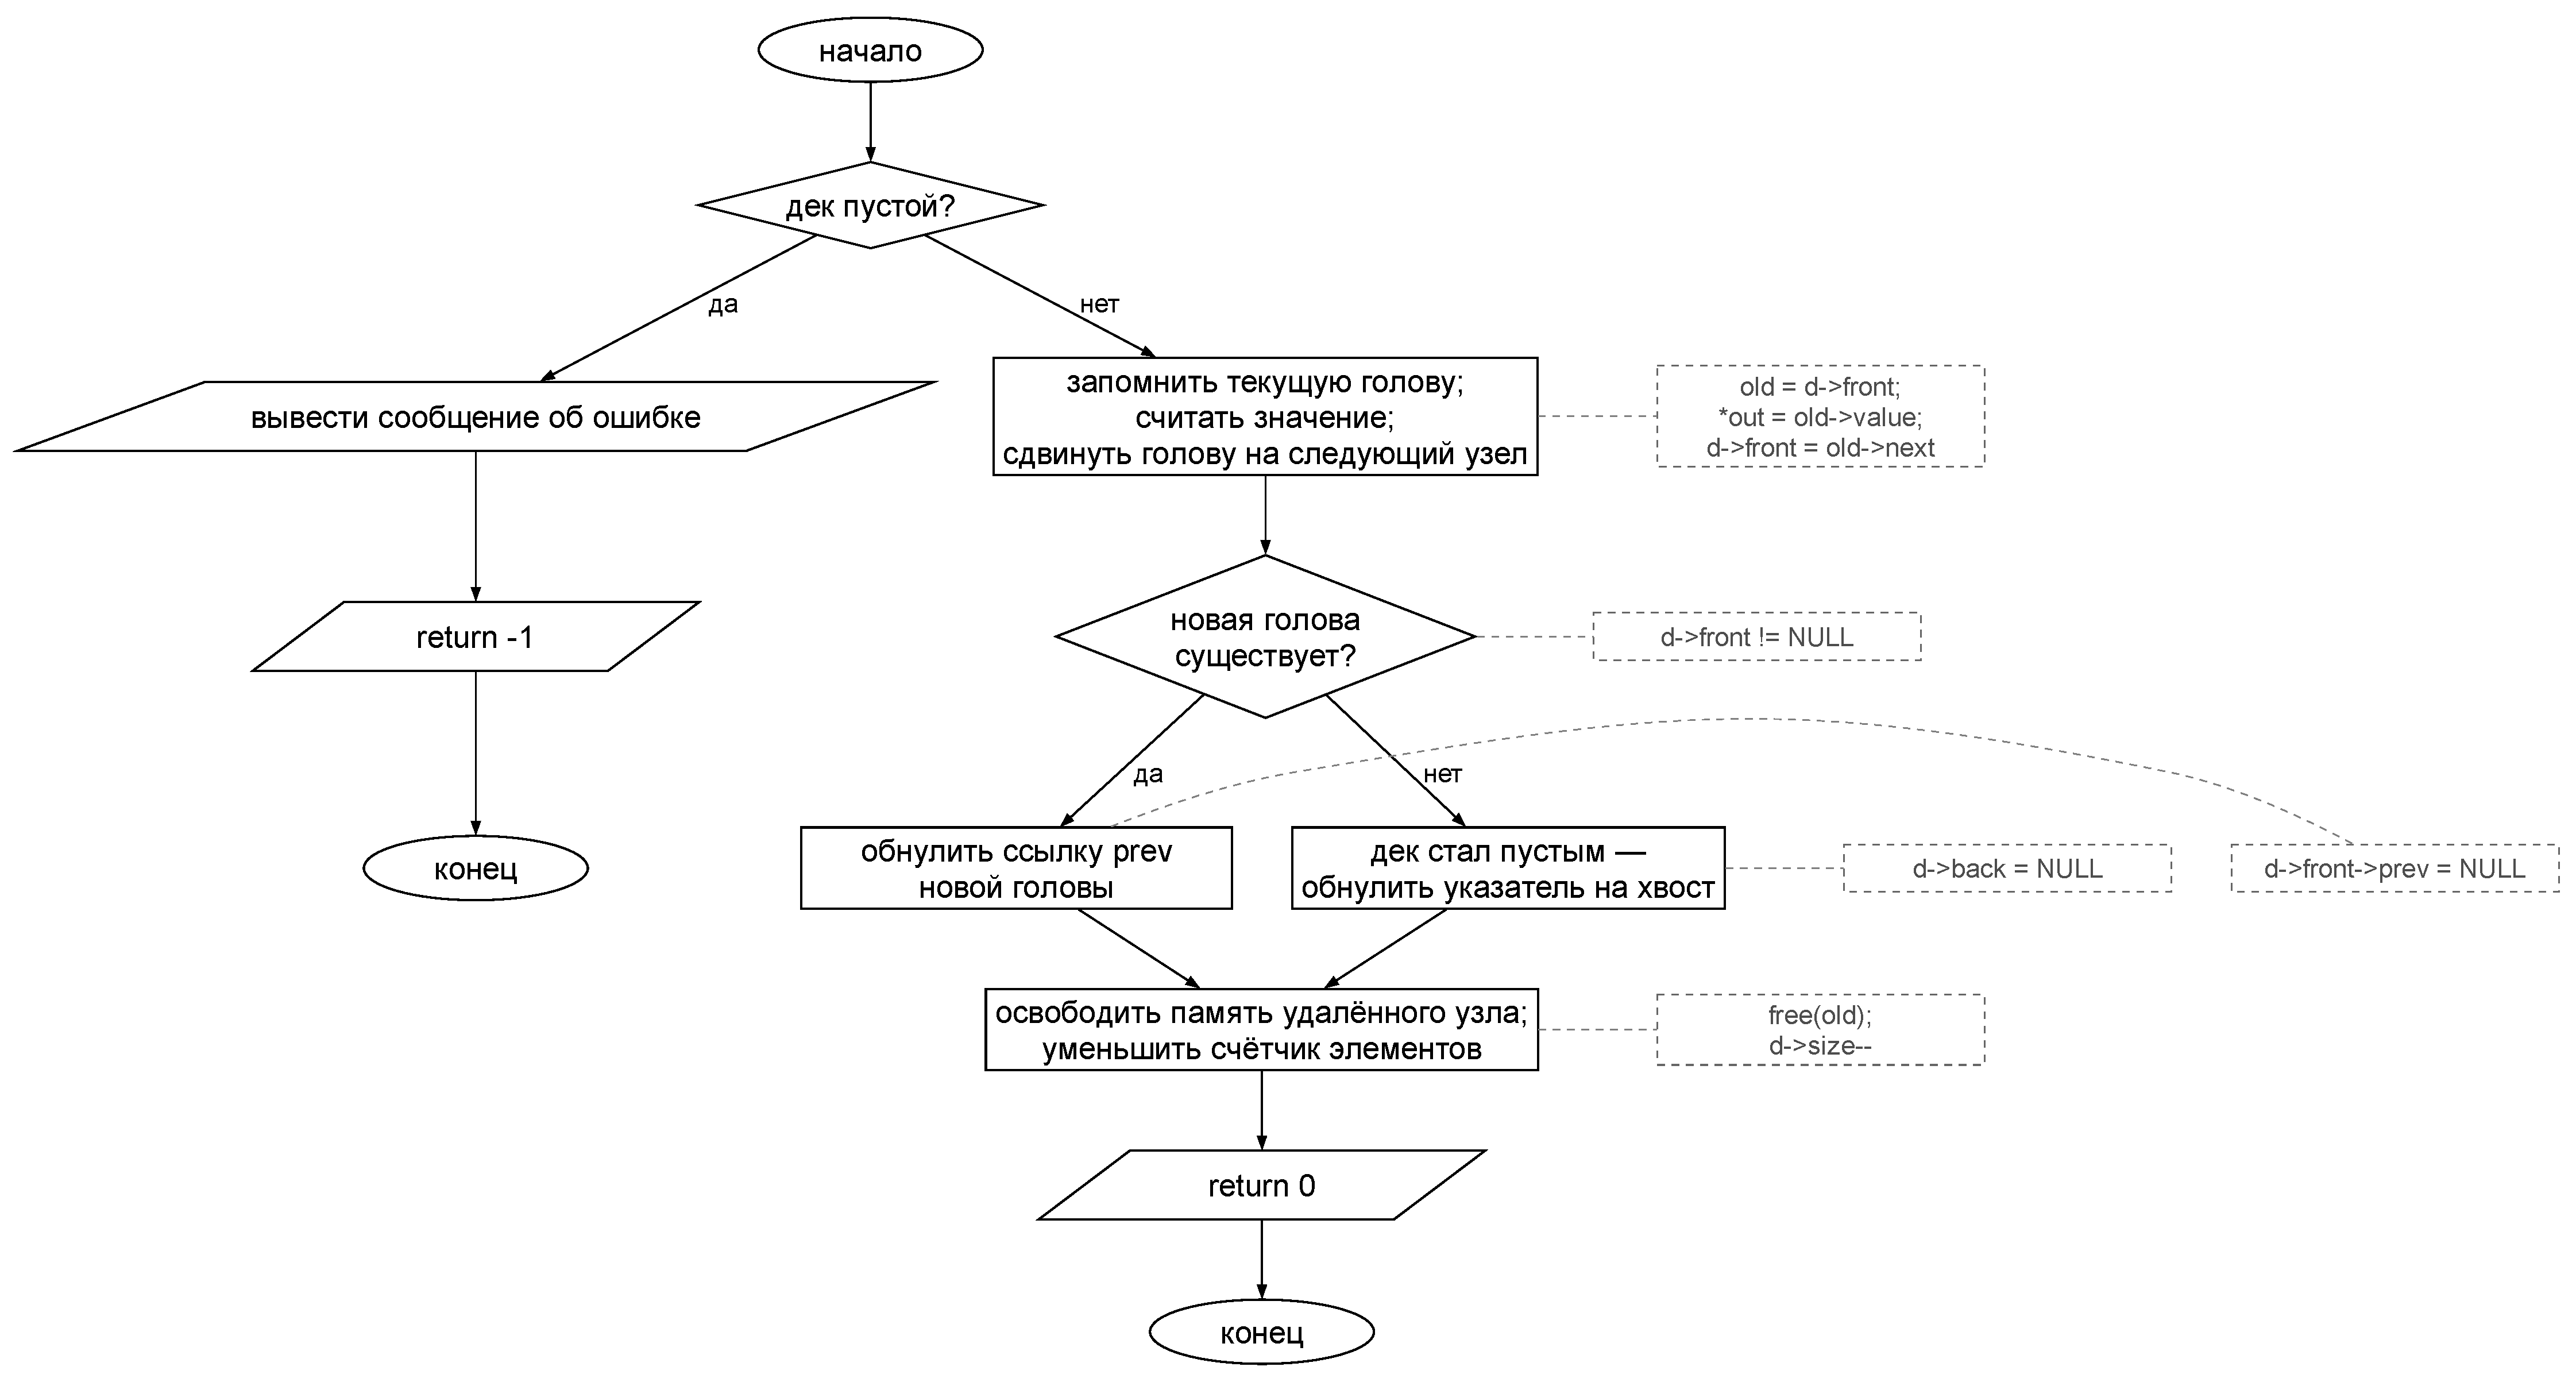
\includegraphics[width=250mm,height=155mm,keepaspectratio]{flowcharts/5c_pop_front.pdf}}
\caption{Извлечение из головы дека (pop\_front)}
\end{figure}
\clearpage

\begin{figure}[H]
\centering
\makebox[\linewidth][c]{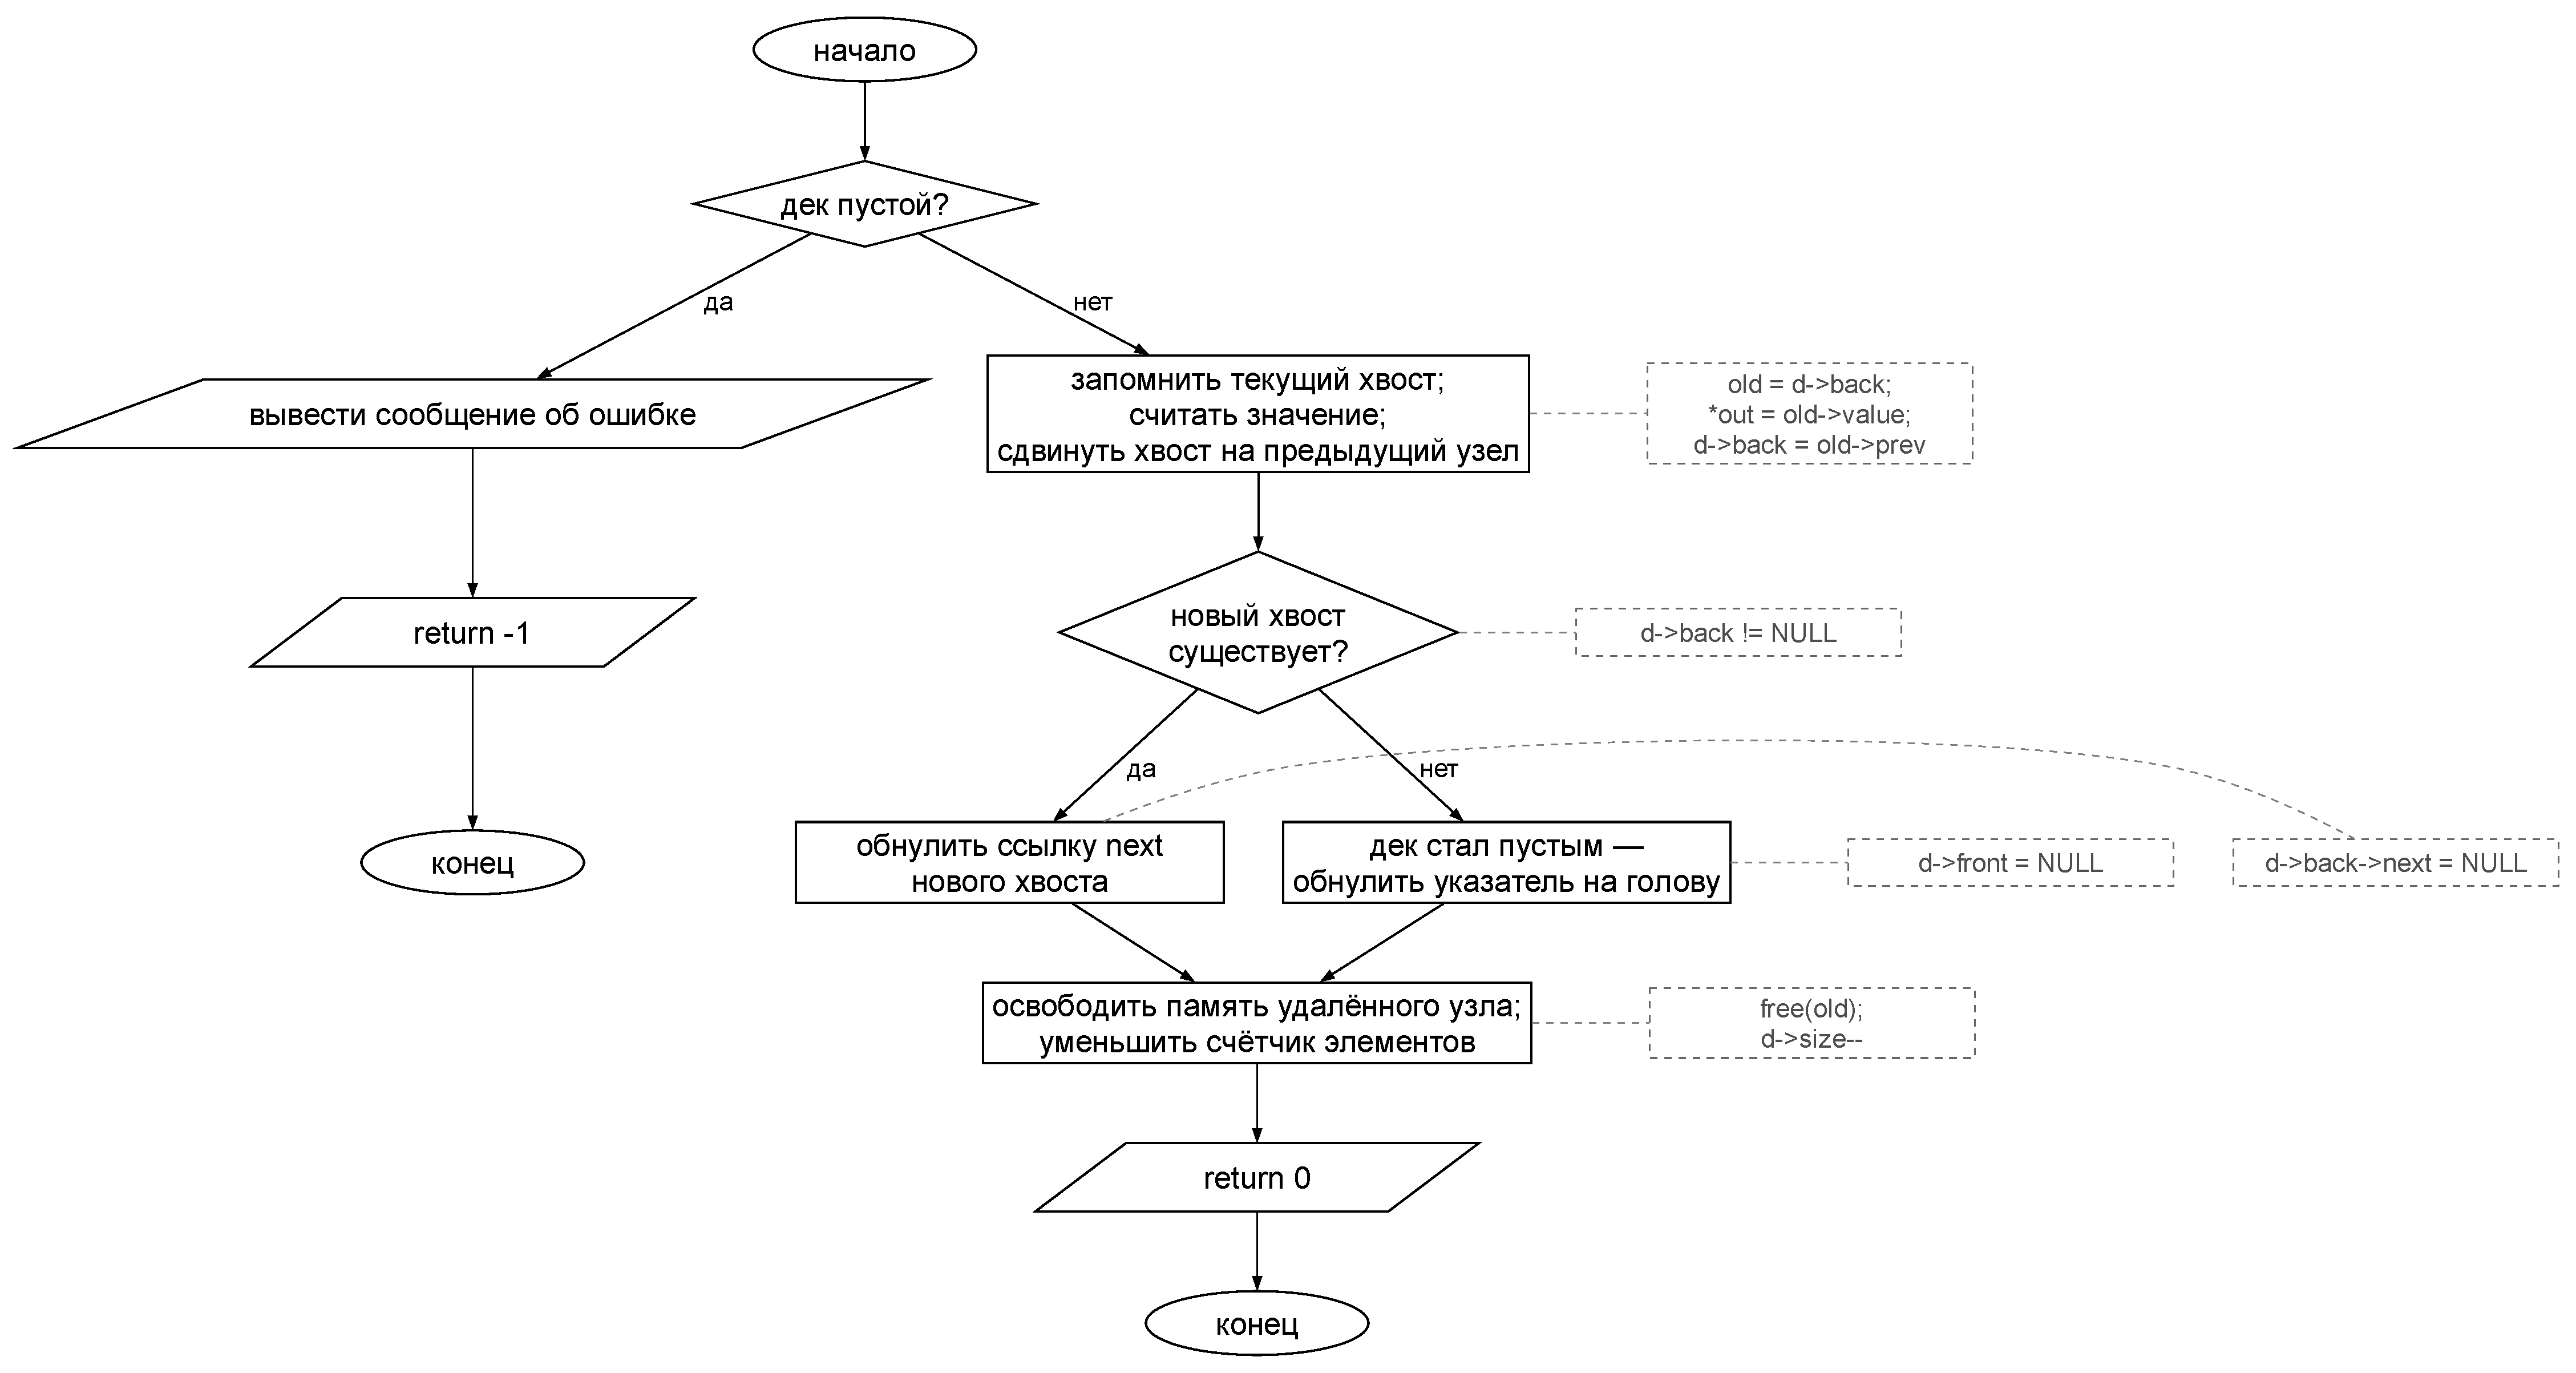
\includegraphics[width=250mm,height=155mm,keepaspectratio]{flowcharts/5d_pop_back.pdf}}
\caption{Извлечение из хвоста дека (pop\_back)}
\end{figure}
\clearpage

\begin{figure}[H]
\centering
\makebox[\linewidth][c]{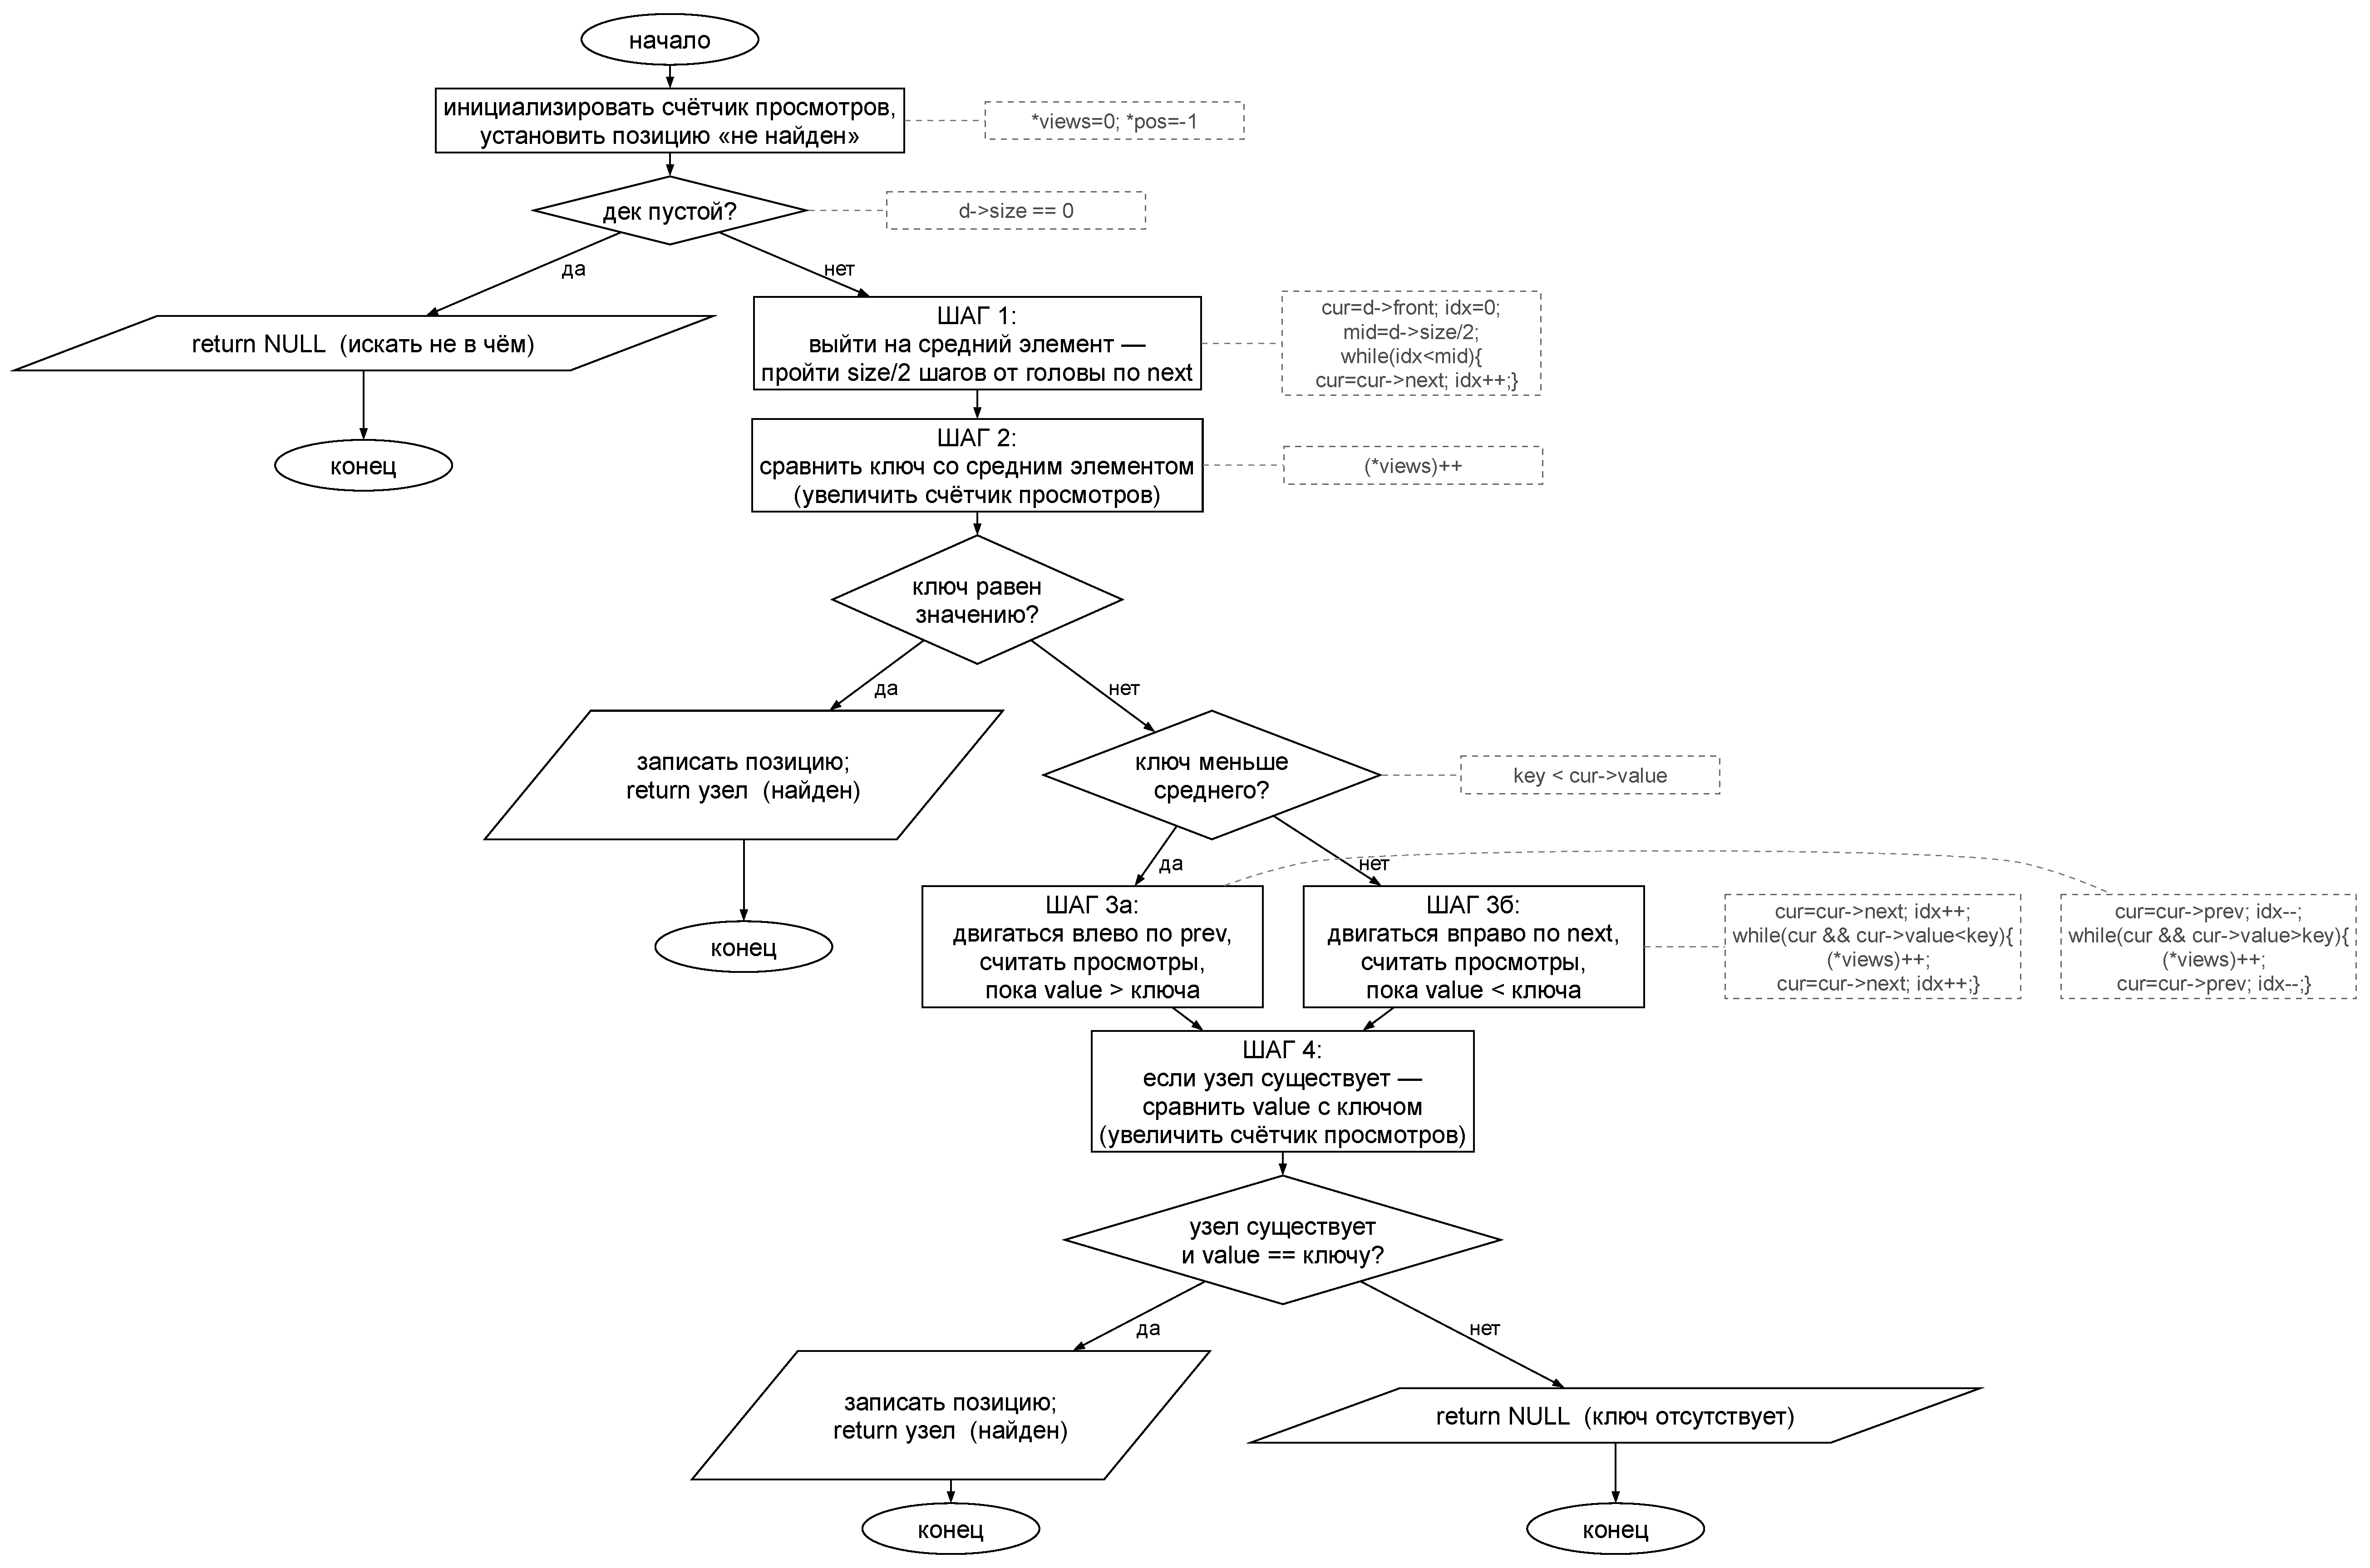
\includegraphics[width=250mm,height=155mm,keepaspectratio]{flowcharts/6_wright_search.pdf}}
\caption{Поиск методом Райта (wright\_search)}
\end{figure}

\end{landscape}

\end{document}
